%% tese_lncc.tex
%%
%% A última versão deste modelo está em
%%   https://github.com/equipe-customizacao-tese-lncc/tese_lncc
%%
%% Criado por:
%% Weslley da Silva Pereira
%% Lucas dos Santos Fernandez
%% Fortià Vila Verges
%%
%% Modificado por:
%% Equipe de customização - Fortià Vila Verges,
%%   Lucas dos Santos Fernandez, Weslley da Silva Pereira
%%
%% Este trabalho consiste de tese_lncc.tex,
%% abntex2lncc.sty e bibliografia.bib
%%

% ------------------------------------------------------------------------
% ------------------------------------------------------------------------
% Modelo de Trabalho Academico (tese de doutorado, dissertacao de
% mestrado e trabalhos monograficos em geral) em conformidade com
% ABNT NBR 14724:2011: Informacao e documentacao - Trabalhos academicos -
% Apresentacao
% ------------------------------------------------------------------------
% ------------------------------------------------------------------------

\documentclass[
	% -- opções da classe memoir --
	12pt,				% tamanho da fonte
	openright,			% capítulos começam em pág ímpar (insere página vazia caso preciso)
	oneside,			% para impressão em frente e verso use twoside
	a4paper,			% tamanho do papel.
	% -- opções da classe abntex2 --
	%chapter=TITLE,		% títulos de capítulos convertidos em letras maiúsculas
	%section=TITLE,		% títulos de seções convertidos em letras maiúsculas
	%subsection=TITLE,	% títulos de subseções convertidos em letras maiúsculas
	%subsubsection=TITLE,% títulos de subsubseções convertidos em letras maiúsculas
	sumario=tradicional,% sumário tradicional, com tabulação
	% -- opções do pacote babel --
	brazil,			% idioma adicional para hifenização
	french,				% idioma adicional para hifenização
	spanish,			% idioma adicional para hifenização
	english				% o último idioma é o principal do documento (mude se precisar)
	]{abntex2}

% ---
% Pacotes básicos
% ---
\usepackage{lmodern}			% Usa a fonte Latin Modern			
\usepackage[T1]{fontenc}		% Selecao de codigos de fonte.
\usepackage[utf8]{inputenc}		% Codificacao do documento (conversão automática dos acentos)
\usepackage{lastpage}			% Usado pela Ficha catalográfica
\usepackage{indentfirst}		% Indenta o primeiro parágrafo de cada seção.
\usepackage{color}				% Controle das cores
\usepackage{graphicx}			% Inclusão de gráficos
\usepackage{microtype} 			% para melhorias de justificação
\usepackage{abntex2lncc}		% Formatacao especifica do modelo do LNCC
\usepackage{booktabs}
\usepackage[table,xcdraw]{xcolor}
\usepackage{amssymb}
\usepackage{tcolorbox}
\usepackage{algorithm}
\usepackage[noend]{algpseudocode}
\usepackage{svg}
\usepackage{mathtools,bm}
\usepackage{listings}
\lstset{language=R}
\usepackage{amsthm}

\theoremstyle{plain}
\newtheorem{thm}{Theorem}[chapter] % reset theorem numbering for each chapter

\theoremstyle{definition}
\newtheorem{defn}[thm]{Definition} % definition numbers are dependent on theorem numbers
\newtheorem{exmp}[thm]{Example} % same for example numbers

%\usepackage[colorlinks=true,linkcolor=blue,urlcolor=black,bookmarksopen=true]{hyperref}
% ---
		
% ---
% Pacotes adicionais, usados apenas no âmbito do Modelo Canônico do abnteX2
% ---
%\usepackage{lipsum}				% para geração de dummy text
% ---

% ---
% Pacotes de citações
% ---
\usepackage[brazilian,hyperpageref]{backref}	 % Paginas com as citações na bibl
\usepackage[alf]{abntex2cite}	% Citações padrão ABNT
\usepackage{multirow}           % permite mesclar linhas e colunas em tabelas

\usepackage{pst-uml}

% ---
% CONFIGURAÇÕES DE PACOTES
% ---

% ---
% Configurações do pacote backref
% Usado sem a opção hyperpageref de backref
\renewcommand{\backrefpagesname}{Citado na(s) página(s):~}
% Texto padrão antes do número das páginas
\renewcommand{\backref}{}
% Define os textos da citação
\renewcommand*{\backrefalt}[4]{
	\ifcase #1 %
		Nenhuma citação no texto.%
	\or
		Citado na página #2.%
	\else
		Citado #1 vezes nas páginas #2.%
	\fi}%
% ---

% ---
% CONFIGURAÇÕES DE USUÁRIO
% ---
	
% ---
% Pasta principal de imagens e logo do LNCC
\graphicspath{img}
\logoLNCC{logo/lncc}
% ---

% ---
% Tipo de trabalho (apenas uma das opções abaixo deve estar descomentada)
%\dissertacaoMestrado
\teseDoutorado
% ---

% ---
% Título
\titulo{Generalized Lambda Distribution for Uncertainty Quantification of Large-scale Spatio-temporal Models}
% Nome do aluno
\nomeAutor{Noel}{Moreno Lemus}
% Nome do orientador
\nomeOrientador{Fábio André}{Machado Porto}
% Coorientador(es)
% \coorientador{José Oliveira Pereira}
%\coorientador[Coorientadores:]{Coorientador 1 e Coorientador 2}
% ---

% ---
% Local
\local{Petrópolis, RJ - Brasil}
% Data
\data{Abril de 2018}
% Instituição
\instituicao{%
  Laboratório Nacional de Computação Científica
  \par
  Programa de Pós-Graduação em Modelagem Computacional}
% ---

% ---
% O preambulo deve conter o tipo do trabalho, o objetivo,
% o nome da instituição e a área de concentração
% portugues
%\preambulo{\tipoTrabalho submetida ao corpo docente do Laboratório Nacional de Computação Científica como parte dos requisitos necessários para a obtenção do grau de \grau em Ciências em Modelagem Computacional.}
%ingles
\preambulo{\tipoTrabalho submitted to the examining committee in partial fulfillment of the requirements for the degree of \grau of Sciences in Computational Modeling.}
% ---

% ---
% FICHA CATALOGRÁFICA
%
% Representa o código que sua tese/dissertação terá nos registros de  nossa biblioteca.
%
% Observação: Ao terminar de escrever sua tese/dissertação e a mesma for aprovada pela comissão de avaliação para a defesa, favor se dirigir a biblioteca.
% ---
\codebib{XXX.XXX}
\codetese{XXXX}
% ---

% ---
% Configurações de aparência do PDF final

\definecolor{blue}{RGB}{41,5,195}

% informações do PDF
\makeatletter
\hypersetup{
     	%pagebackref=true,
		pdftitle={\@title},
		pdfauthor={\@author},
    	pdfsubject={\imprimirpreambulo},
	    pdfcreator={LaTeX with abnTeX2},
		pdfkeywords={abnt}{latex}{abntex}{abntex2}{trabalho acadêmico},
		colorlinks=true,       		% false: boxed links; true: colored links
    	linkcolor=blue,          	% color of internal links
    	citecolor=blue,        		% color of links to bibliography
    	filecolor=magenta,      		% color of file links
		urlcolor=blue,
		bookmarksdepth=4
}
\makeatother
% ---

% ---
% Espaçamentos entre linhas e parágrafos
% ---

% O tamanho do parágrafo é dado por:
\setlength{\parindent}{1.3cm}

% Controle do espaçamento entre um parágrafo e outro:
\setlength{\parskip}{0.2cm}  % tente também \onelineskip

% ---
% compila o indice
% ---
\makeindex
% ---

% ----
% Início do documento
% ----

\begin{document}

% Seleciona o idioma do documento (conforme pacotes do babel)
\selectlanguage{english}
%\selectlanguage{brazil}

% Retira espaço extra obsoleto entre as frases.
\frenchspacing

% ----------------------------------------------------------
% ELEMENTOS PRÉ-TEXTUAIS
% ----------------------------------------------------------
% \pretextual

% ---
% Capa
% ---
\imprimircapa
% ---

% ---
% Folha de rosto
% (o * indica que haverá a ficha bibliográfica)
% ---
\imprimirfolhaderosto*
% ---

% ---
% Inserir a ficha bibliografica
% ---

% Isto é um exemplo de Ficha Catalográfica, ou ``Dados internacionais de
% catalogação-na-publicação''. Você pode utilizar este modelo como referência.
% Porém, provavelmente a biblioteca da sua universidade lhe fornecerá um PDF
% com a ficha catalográfica definitiva após a defesa do trabalho. Quando estiver
% com o documento, salve-o como PDF no diretório do seu projeto e substitua todo
% o conteúdo de implementação deste arquivo pelo comando abaixo:
%
% \begin{fichacatalografica}
%     \includepdf{fig_ficha_catalografica.pdf}
% \end{fichacatalografica}

\begin{fichacatalografica}
	\sffamily
	\vspace*{\fill}					% Posição vertical
	\begin{center}					% Minipage Centralizado
	\fbox{
	\begin{minipage}[c][5cm][t]{1.5cm}
	\small
	\imprimirCodeTese
	\end{minipage}
	\begin{minipage}[c][8cm][c]{13.5cm}		% Largura
	\small
	\imprimirUltimoSobrenome,{ }\imprimirNomeAutor
	%Sobrenome, Nome do autor
	
	\hspace{0.5cm} \imprimirtitulo{ }/ \imprimirautor. --
	\imprimirlocal, \imprimirdata-
	
	\hspace{0.5cm} \pageref{LastPage} p. : il. \pagColoridas ; 30 cm.\\
	
	\hspace{0.5cm} \imprimirOrientadoresRotulo~\imprimirorientador
	{ e }\imprimircoorientador\\
	
	\hspace{0.5cm}
	\parbox[t]{\textwidth}{\imprimirtipotrabalho~--~\imprimirinstituicao,
	\imprimirdata.}\\
	
	\hspace{0.5cm}
		1. Uncertainty Quantification.
		2. Big Data.
		3. Information Entropy.
		I. \imprimirUltimoSobrenomeOrientador,{ }\imprimirNomeOrientador.
		II. LNCC/MCTI.
		III. \labelTitulo

	\begin{center}
		CDD: \imprimirCodeBib	
	\end{center}		
	\end{minipage}}
	
	\end{center}
\end{fichacatalografica}
% ---

% ---
% Inserir folha de aprovação
% ---

% Isto é um exemplo de Folha de aprovação, elemento obrigatório da NBR
% 14724/2011 (seção 4.2.1.3). Você pode utilizar este modelo até a aprovação
% do trabalho. Após isso, substitua todo o conteúdo deste arquivo por uma
% imagem da página assinada pela banca com o comando abaixo:
%
% \includepdf{folhadeaprovacao_final.pdf}
%
\begin{folhadeaprovacao}

  \begin{center}
    {\ABNTEXchapterfont\large\imprimirautor}

    \vspace*{\fill}\vspace*{\fill}
    \begin{center}
      \ABNTEXchapterfont\bfseries\Large\imprimirtitulo
    \end{center}
    \vspace*{\fill}

    \hspace{.45\textwidth}
    \begin{minipage}{.5\textwidth}
        \imprimirpreambulo
    \end{minipage}%
    \vspace*{\fill}
   \end{center}

   \aprovadaPor

   \assinatura{\textbf{Prof. \imprimirorientador, D.Sc.} \\ (Presidente)}
   \assinatura{\textbf{Prof. Fernando Alves Rochinha, D.Sc.}}
   \assinatura{\textbf{Prof. Hugo de La Cruz, Ph.D.}}
   \assinatura{\textbf{Prof. Artur Ziviani, Ph.D.}}
   %\assinatura{\textbf{Prof. Patrick Valduriez, Ph.D.}}

   \begin{center}
    \vspace*{0.5cm}
    {\large\imprimirlocal}
    \par
    {\large\imprimirdata}
    \vspace*{1cm}
  \end{center}

\end{folhadeaprovacao}
% ---

% ---
% Dedicatória
% ---
\begin{dedicatoria}
   \vspace*{\fill}
   \vspace*{10cm}
   \flushright
   \noindent
   \textbf{\dedicatorianame\\}
   \textit{To my little and special family.\\} \vspace*{\fill}
\end{dedicatoria}
% ---

% ---
% Agradecimentos
% ---
\begin{agradecimentos}
O autor manifesta reconhecimentos às pessoas e instituições que colaboraram para a execução de seu trabalho.

\end{agradecimentos}
% ---

% ---
% Epígrafe
% ---
\begin{epigrafe}
    \vspace*{\fill}
	\begin{flushright}
		\textit{``Essentially, all models are wrong, but some are useful.''\\
		(George Edward Pelham)}
	\end{flushright}
\end{epigrafe}
% ---

% ---
% RESUMOS
% ---

% resumo no idioma principal
\setlength{\absparsep}{18pt} % ajusta o espaçamento dos parágrafos do resumo
\begin{resumo}
 Segundo a \citeonline[3.1-3.2]{NBR6028:2003}, o resumo deve ressaltar o
 objetivo, o método, os resultados e as conclusões do documento. A ordem e a extensão
 destes itens dependem do tipo de resumo (informativo ou indicativo) e do
 tratamento que cada item recebe no documento original. O resumo deve ser
 precedido da referência do documento, com exceção do resumo inserido no
 próprio documento. (\ldots) As palavras-chave devem figurar logo abaixo do
 resumo, antecedidas da expressão Palavras-chave:, separadas entre si por
 ponto e finalizadas também por ponto.

 \textbf{\palavrasChave}: latex. abntex. editoração de texto.
\end{resumo}

% resumo em inglês
\begin{resumo}[Abstract]
 \begin{otherlanguage*}{english}
 Large-scale spatio-temporal simulations with quantified uncertainty enable scientists/decision-makers to precisely assess the degree of confidence of their simulation-based predictions. This uncertainty could be qu antified or characterized in different ways, from the use of low order statistical moments (the most commonly used), to the evaluation of a complete PDF (a most complete approach). The latter provides a more comprehensive description of the uncertainty leading to aware decisions. However, fitting PDFs to the data is computational intesive. Moreover, due to heterogeneity the uncertainty computed in regions of the dataset is hampered by the existence of different PDF types. 
 
 In this thesis, we propose a new method to quantify the uncertainty in large-scale spatio-temporal models based on the Generalized Lambda Distribution (GLD). GLD is a family of PDFs that nicely models
the heterogeneity of uncertainty as discussed above. It is specified by 4 parameters that
simplifies PDFs comparisons easing analytical processing, such as clustering. We show how
the dataset modeled through GLDs can be used to answer queries, such as: (\textit{i}) how to
group the output of the UQ process based on the simillarity of the uncertainty?, (\textit{ii}) what
is the uncertainty in some spatio-temporal locations not previously analysed?, (\textit{iii}) what is
the uncertainty of an specific spatio-temporal region?, (\textit{iv}) how to compare two regions as a
function of its uncertainty?, and (\textit{v}) what is the less uncertain model from a set of models?
The proposed method has been tested in realistic use cases from various scientific areas.
Additionally, an R package has been implemented with all the functionalities discussed in
the thesis.
 
   \textbf{Keywords}: Uncertainty Quantification, Large-scale spatio-temporal models, Big Data, Generalized Lambda Distribution
 \end{otherlanguage*}
\end{resumo}

%% resumo em português-br
%\begin{resumo}[Resumo]
% \begin{otherlanguage*}{brazil}
%    Este é um resumo em português do Brasil.
%
%   \textbf{Palavras-chave}: latex. abntex. editoração de texto.
% \end{otherlanguage*}
%\end{resumo}

%% resumo em francês
%\begin{resumo}[Résumé]
% \begin{otherlanguage*}{french}
%    Il s'agit d'un résumé en français.
%
%   \textbf{Mots-clés}: latex. abntex. publication de textes.
% \end{otherlanguage*}
%\end{resumo}

%% resumo em espanhol
%\begin{resumo}[Resumen]
% \begin{otherlanguage*}{spanish}
%   Este es el resumen en español.
%
%   \textbf{Palabras clave}: latex. abntex. publicación de textos.
% \end{otherlanguage*}
%\end{resumo}
% ---

% ---
% inserir lista de figuras
% ---
\pdfbookmark[0]{\listfigurename}{lof}
\listoffigures*
\cleardoublepage
% ---

% ---
% inserir lista de tabelas
% ---
\pdfbookmark[0]{\listtablename}{lot}
\listoftables*
\cleardoublepage
% ---

% ---
% inserir lista de abreviaturas e siglas
% ---
\begin{siglas}
  \item[UQ] Uncertainty Quantification
  \item[FP] Forward Problem
  \item[\textit{QoI}] Quantity of Interest
  \item[\textit{GLD}] Generalized Lambda Distribution
  \item[\textbf{p.f.}] percentile function
  \item[\textbf{r.v.s}] random variables
  \item[GLDEX] r package to compute the GLD 
  \item[M\&S] Modeling and Simulation
\end{siglas}
% ---

% ---
% inserir lista de símbolos
% ---
\begin{simbolos}
  \item[$ \Gamma $] Letra grega Gama
  \item[$ \Lambda $] Lambda
  \item[$ \zeta $] Letra grega minúscula zeta
  \item[$ \in $] Pertence
\end{simbolos}
% ---

% ---
% inserir o sumario
% ---
\pdfbookmark[0]{\contentsname}{toc}
\tableofcontents*
\cleardoublepage
% ---


% ----------------------------------------------------------
% ELEMENTOS TEXTUAIS
% ----------------------------------------------------------
\textual

% ----------------------------------------------------------
% Capítulos
% ----------------------------------------------------------
\chapter[Introduction]{Introduction}\label{cap:intro}
The rapid growth of high-performance computing and the advances in numerical techniques in the last two decades have provided an unprecedented opportunity to explore complex physical phenomena using large-scale spatio-temporal modeling and simulation.  At the same time, scientific community is leaving behind the traditional deterministic approach, which offers  point predictions with no associated uncertainty \cite{Johnstone2015};  to include Uncertainty Quantification (\textit{UQ}) as a common practice in their researches. 

Large-scale spatio-temporal simulations with quantified uncertainty enable scientists to make precise statements about the degree of confidence they have in their simulation-based predictions. These approaches find practical applicability in models for predicting the behavior of weather, hurricane forecasts \cite{Tobergte2013}, subsurface hydrology \cite{Baroni2014a}, geology \cite{Guerra2016}, nuclear reactor design, financial portfolios \cite{Chen2008}, and biological phenomena, just to name a few. They also allow to study physical phenomena that are impossible to assess experimentally, for example: simulate nuclear accidents, or the conditions that some spatial vehicle will find at landing in Mars, and so on. The success of these techniques has made them increasingly important tools for high impact predictions and decision making.

\textit{UQ}  includes different aspects that warranty the predictive fidelity of a numerical simulation, such as the uncertainty in the experimental data, which is used for defining the parameter values of a model; the propagation of uncertain  parameters through the model; and the choice of the model itself. \textit{UQ} is a complex process that covers the following main tasks: (i) uncertainty characterization \cite{Crespo2014}, also called model calibration \cite{Farrell2015a} or statistical inverse problem \cite{Estacio-Hiroms2012};  (ii) sensitivity analysis; (iii) forward problem or uncertainty propagation; and (iv) model selection.

This paper is focused on  \textit{forward propagation}, whose objective is to quantify the uncertainties in model output(s) propagated from uncertain inputs. The targets of \textit{forward propagation} analysis can be: (i) evaluate low-order moments ( i.e. mean and variance) of the outputs, (ii) evaluate the reliability of the outputs, and/or (iii) assess the complete probability distribution (\textit{PDF}) of the outputs.

When dealing with large-scale spatio-temporal models, a huge among of data is generated as a result of the simulation process. Indeed, on each spatio-temporal location $(s_{i},t_{j}) \in \mathcal{S} \times \mathcal{T}\subseteq\mathbb{R}^{3}\times\mathbb{R}$ , usually more than $10^4$ simulations are performed. Then, the size of the output dataset is in the order of $N_{s}\times N_{t}\times N_{sim}$, where: $N_{s}$ is the number of spatial locations, $N_{t}$ is the number of time steps, and $N_{sim}$ is the number of simulations.  An example of the volume of data generated by these simulations is given in the experimental section \ref{Experiments} of this paper, where the output dataset is about 2.4 TB. This turn \textit{forward propagation} in a data intensive problem.

Another important aspect, which is often not taken into account, is that the uncertainty need to be quantified in some way that can be used after, to answer questions that arise in the \textit{UQ} context. In that sense, assess the complete \textit {PDF} could be the best way to quantify uncertainty, because if you can find the \textit {PDF} that best fit the dataset with reasonably accurately, you can get all the statistical properties under one roof. At the same time, we can substitute the original data by the \textit {PDFs}, which represents a huge reduction in the volume of data to manipulate.

Contradictorily, statistical moments (e.g. mean and standard deviation) are possibly the most used ways to quantify the uncertainty, despite the fact that they doesn't have information about the manner in which the data are distributed \cite{Lampasi2006}. This is because of the difficulty to find the \textit{PDF} that best fit a dataset \cite{Karian2011},  even more, when dealing with large-scale spatio-temporal models where the \textit{PDF} needs to be derived on each spatio-temporal location, and therefore the  \textit{forward propagation} problem becomes time consuming and computationally intensive too.

However, the use of low order moments alone prevents us from making accurate analysis with respect to the uncertainty. They are not enough neither for the characterization nor for the quantification of the uncertainty, and questions such as:
\begin{itemize}
\item What is the uncertainty in the spatio-temporal region $\mathcal{S}_{i} \times \mathcal{T}_{j}$ associated to the \textit{QoI} 
$q_{k}$  and a computational model $\mathcal{M}_{m}$?
\item How to compare different spatio-temporal regions $\mathcal{S}_{i} \times \mathcal{T}_{j}$ with respect to the uncertainty? 
\item What is the less uncertain model from the set of models $\mathcal{M}={\mathcal{M}_{1},\mathcal{M}_{2},
....\mathcal{M}_{m}}$, to predict the value of a QoI $q_{k}$, over a spatio-temporal region $\mathcal{S}_{i} \times \mathcal{T}_{j}$?
\end{itemize}
can be poorly answered. So, we emphasize that only the characterization of the uncertainty by using the \textit{PDF} allows aware decisions.

A first effort to try to estimate the \textit{PDFs} on large-scale spatio-temporal simulations was done by \cite{Liu2018} {Ji et. al.} in \textbf{\textit{Parallel Computation of PDFs on Big Spatial Data Using Spark}}. They propose a new solution to efficiently compute the \textit{PDFs} in parallel using Spark, through three methods: data grouping, machine learning prediction and sampling. The main drawback of the proposed approach is that you should try many different distributions, to find the PDF that best fits the dataset on each specific spatio-temporal location. Another drawback is that, as we mentioned above, the uncertainty needs to be quantified in the way that facilitates its further use; and the heterogeneity of the functions used in the approach doesn't facilitate it. 

To face these challenges, in this paper we propose a general framework to quantify the uncertainty in large-scale spatio-temporal models. It uses a data-driven approach and combines the generalized lambda distribution (\textit{GLD}), clusters algorithms and information entropy, for helping researchers to answer the above questions and many others that arise in \textit{UQ} context. Our proposal provides a generally applicable and easy-to-use tool that supports the representation and analysis of uncertainty, as was suggested in the "\textit{Workshop on Quantification, Communication, and Interpretation of Uncertainty in Simulation and Data Science}" \cite{Tobergte2013}. 

In order to illustrate the use of the proposed framework, a case study is discussed. The main results obtained are: (i) the \textit{GLD} good fits for more than the 80 \% of the dataset, (ii) the use of the \textit{GLD} allows to include clustering algorithms to group the spatio-temporal locations with similar uncertainty, (iii) the centroids  of the clusters can be used as a faithful representation of the rest of the spatio-temporal locations, which significantly reduces the data corresponding to the simulation outputs, (iv) with the use of these centroids we can characterize the uncertainty in any spatio-temporal region as a mixture of \textit{GLDs}.

The rest of the paper is organized as follows: Section \ref{UQBackground} gives the theoretical foundations of \textit{UQ} and highlights some interesting aspects included in our proposal. Section \ref{materials_methods} describes the principal characteristics of the \textit{GLD} that make it suitable for this proposal. Section \ref{Approach} presents the proposed approach, the workflow we implement and some considerations of the implementation. Section \ref{Experiments} presents a use case and discusses the results. This use case allows us to explain our approach in the context of a real problem, which facilitates its understanding. Section \ref{RelatedWorks} covers the related works and finally, section \ref{Conclusions} concludes the paper and proposes some future works.

\section{Research Objectives}

\begin{tcolorbox}
The main objective of this thesis is the proposal of a new method to quantify the uncertainty in large-scale spatio-temporal models based on the Generalized Lambda Distribution (GLD).
\end{tcolorbox}

To achieve that goal the following research questions need to be answered:

\textbf{RQ1.} how to group the output of the UQ process based on the similarity of the uncertainty?

\textbf{RQ2.} what is the uncertainty in some spatio-temporal locations not previously analysed?

\textbf{RQ3.} what is the uncertainty of an specific spatio-temporal region?

\textbf{RQ4.} how to compare two regions as a function of its uncertainty?

\textbf{RQ5.} what is the less uncertain model from a set of models?

\textbf{RQ1} and \textbf{RQ2} are answered in chapter \ref{cap:gld_clustering}, while \textbf{RQ3}, \textbf{RQ4} and \textbf{RQ5} are answered in chapter \ref{cap:our_approach}. In chapter \ref{cap:use_cases} all the questions are answered again for all the use cases.

\section{Highlights of the Dissertation}

\section{Organization of the Dissertation}

The structure of the remainder of this thesis is outlined for reference.

\textbf{Chapter 2} background of UQ.

\textbf{Chapter 3} Ji paper.

\textbf{Chapter 4} GLD.

\textbf{Chapter 5} GLD clustering and kriging.

\textbf{Chapter 6} Workflow.

\textbf{Chapter 7} Use cases.

\textbf{Chapter 8} Conclusions and future works.

%% abtex2-modelo-include-comandos.tex, v-1.9.6 laurocesar
%% Copyright 2012-2016 by abnTeX2 group at http://www.abntex.net.br/
%%
%% This work may be distributed and/or modified under the
%% conditions of the LaTeX Project Public License, either version 1.3
%% of this license or (at your option) any later version.
%% The latest version of this license is in
%%   http://www.latex-project.org/lppl.txt
%% and version 1.3 or later is part of all distributions of LaTeX
%% version 2005/12/01 or later.
%%
%% This work has the LPPL maintenance status `maintained'.
%%
%% The Current Maintainer of this work is the abnTeX2 team, led
%% by Lauro César Araujo. Further $\infty$ormation are available on
%% http://www.abntex.net.br/
%%
%% This work consists of the files abntex2-modelo-include-comandos.tex
%% and abntex2-modelo-img-marca.pdf
%%

% ---
% Este capítulo, utilizado por diferentes exemplos do abnTeX2, ilustra o uso de
% comandos do abnTeX2 e de LaTeX.
% ---

\chapter{Uncertainty Quantification Background}\label{cap:backgroud}


\begin{flushright}
	\textit{``UQ cannot tell you that your model is 'right' or 'true', \\
	but only that, if you accept the validity of the model (to some \\
	quantified degree), then you must logically accept the validity\\
	of certain conclusions (to some quantified degree)''\\
	\cite{Sullivan2015}}
\end{flushright}

Uncertainty quantification (UQ) is a topic of great importance and hence widespread interest in computational analyses that are used to support important societal decisions on issues related to climate change [15-19], reactor safety [20-26], radioactive waste disposal [27-34], nuclear weapon safety [35-38], economic policy [39-43], environmental degradation [44- 47], and many additional areas of concern and challenge. Indeed, it is difficult to envision how adequately informed decisions can be made on such issues without an appropriate assessment of the uncertainties present in the supporting analyses.

In this chapter, we summarize some definitions in UQ context that are important to understand the rest of the document. Also, different ways of representation of the uncertainty are discussed, with a brief justification of those we are going to use in the thesis. A general workflow of the UQ process is presented where we contextualize our contributions. A detailed discussion about forward propagation is presented. And finally, we summarize the chapter.

All results of interest can be derived from the PDF \cite{Cox2012}.

In particular it is not always convenient to retain the M = 106, say, (vector) values produced by MC and use them subsequently \cite{Cox2012}.

\section{Definitions}
\subsection{Errors vs Uncertainties}

The mismatch between the true physical phenomena and the prediction obtained by modeling and simulation (M\&S) process can arise from the mathematical representation of a real problem, a physical problem (are the values of the parameters a good representation of the reality?), a computational problem (translation of a mathematical formulation into a numerical algorithm and a computational code) \cite{Thibaut2015}. Uncertainty and error can be considered as the broad categories  that  are  normally  associated to this mismatch. Until recently terms  uncertainty  and error  have  commonly  been  used  interchangeably.  It is believed, however, that failure to distinguish between these terms is detrimental to the quantification of credibility in M\&S. According to \cite{Oberkampf1998} we can classify errors and uncertainties as follow: 

\begin{itemize}
\item[•] \textbf{errors:} recognizable deficiencies of the model or the algorithms employed. Errors are associated to: physical approximations to simplify the modeling of a physical process, translation of the mathematical to computational model, numerical approximations (truncation or roundoff), etc. When the errors are knowns there are reasonable means of estimating the magnitude of the error introduced. 
\item[•] \textbf{uncertainties:} potential deficiency that is due to lack of knowledge. The different sources of uncertainty can be:
\begin{itemize}
\item[-] \textbf{parameter uncertainty}, which comes from the model parameters that are inputs to the computer model (mathematical model) but whose exact values are unknown to experimentalists and cannot be controlled in physical experiments, or whose values cannot be exactly inferred by statistical methods. Examples are the local free-fall acceleration in a falling object experiment, various material properties in a finite element analysis for engineering, and multiplier uncertainty in the context of macroeconomic policy optimization \cite{Kennedy2001}.
\item[-] \textbf{model inadequacy}, no model is perfect. Even if there is no parameter uncertainty, so that we know the true values of all the inputs required to make a particular prediction of the process being modeled, the predicted value will not equal the true value of the process. The discrepancy is model inadequacy. Since the real process may itself exhibit random variability, we define model inadequacy to be the difference between the true mean value of the real world process and the code output at the true values of the inputs.
\item[-] \textbf{parametric variability}, which comes from the variability of input variables of the model. For example, the dimensions of a work piece in a process of manufacture may not be exactly as designed and instructed, which would cause variability in its performance. 
\item[-] \textbf{structural uncertainty}, aka model inadequacy, model bias, or model discrepancy, which comes from the lack of knowledge of the underlying true physics. It depends on how accurately a mathematical model describes the true system for a real-life situation, considering the fact that models are almost always only approximations to reality. One example is when modeling the process of a falling object using the free-fall model; the model itself is inaccurate since there always exists air friction. In this case, even if there is no unknown parameter in the model, a discrepancy is still expected between the model and true physics. 
\item[-] \textbf{algorithmic uncertainty}, aka numerical uncertainty, which comes from numerical errors and numerical approximations per implementation of the computer model. Most models are too complicated to solve exactly. For example, the finite element method or finite difference method may be used to approximate the solution of a partial differential equation, which, however, introduces numerical errors. Other examples are numerical integration and infinite sum truncation that are necessary approximations in numerical implementation. 
\item[-] \textbf{experimental uncertainty}, aka observation error, which comes from the variability of experimental measurements. The experimental uncertainty is inevitable and can be noticed by repeating a measurement for many times using exactly the same settings for all inputs/variables. 
\item[-] \textbf{interpolation uncertainty}, which comes from a lack of available data collected from computer model simulations and/or experimental measurements. For other input settings that don't have simulation data or experimental measurements, one must interpolate or extrapolate in order to predict the corresponding responses.
\end{itemize}
\end{itemize}

A more elegant definition of what uncertainty is, is enunciated in \cite{Helton2009} as:

\begin{defn}
Uncertainty is a best estimate of the range of a particular metric which may derive from one or two broad sources. Uncertainties that reflect a lack of knowledge about the appropriate value to use for a quantity that is assumed to have (missing modifier: a fixed?) value in the context of a particular analysis are termed \textbf{\textit{epistemic}}. Uncertainties that arise from an inherent randomness in the behavior of the system under study are termed \textbf{\textit{aleatoric}}.
\end{defn}

\subsection{Aleatoric vs Epistemic Uncertainty}

It is sometimes assumed that uncertainty can be classified into those two categories, \textbf{\textit{aleatoric}} and \textbf{\textit{epistemic}}, although the validity of this categorization is open to debate \cite{Kiureghian2009}. 

\textbf{Aleatoric uncertainty} arises from an inherent randomness in the properties or behavior of the system under study. For example, the weather conditions at the time of a reactor accident are inherently random with respect to our ability to predict the future. Other examples include the variability in the properties of a population of weapon components and the variability in the possible future environmental conditions that a weapon component could be exposed to. Alternative designations for \textbf{aleatory uncertainty} include variability, stochastic, irreducible and type A. \cite{Helton2009}

\textbf{Epistemic uncertainty} derives from a lack of knowledge about the appropriate value to use for a quantity that is assumed to have a fixed value in the context of a particular analysis. For example, the pressure at which a given reactor containment would fail for a specified set of pressurization conditions is fixed but not amenable to being unambiguously defined. Other examples include minimum voltage required for the operation of a system and the maximum temperature that a system can withstand before failing. Alternative designations for \textbf{epistemic uncertainty} include state of knowledge, subjective, reducible and type B. \cite{Helton2009}

While \textbf{epistemic uncertainty} can be reduced through experiments, improvement of the numerical methods and so on, \textbf{aleatory uncertainty} can not be reduced. 


\subsection{Uncertainty Quantification}

UQ is not a mature field like linear algebra or single-variable complex analysis, with stately textbooks containing well-polished presentations of classical theorems bearing August names like Cauchy, Gauss and Hamilton. Both because of its youth as a field and its very close engagement with applications, UQ is much more about problems, methods and ‘good enough for the job’. There are some very elegant approaches within UQ, but as yet no single, general, overarching theory of UQ. \cite{Sullivan2015}

UQ neither have a unique and globally accepted definition. In the reviewed literature we find some definitions that, from our point of view, are those that batter describe what UQ is.  

In the Wikipedia we find the following definition: 

\begin{defn}
Uncertainty Quantification is the science of quantitative characterization and reduction of uncertainties in applications. It tries to determine how likely certain outcomes are if some aspects of the system are not exactly known.
\end{defn}

This definition is very general and may be ignore some important aspects, by as a first approach is a good one. 

In October of 2009 the U.S. Department of Energy organize a comission to study the impact of Extreme Scale computing in its National Security. One of the aspects analysed by the comision was UQ. In the report \textit{"Scientific Grand Challenges in National Security: The Role of Computing at the Extreme Scale"} \cite{DEnergy2009}, the authors define UQ as:

\begin{defn}
Uncertainty Quantification (UQ) studies all sources of error and uncertainty, including the following:  
systematic and stochastic measurement error; ignorance; limitations of theoretical models; limitations of 
numerical representations of those models; limitations of the accuracy and reliability of computations, 
approximations, and algorithms; and human error. A more precise definition is UQ is the end-to-end 
study of the reliability of scientific inferences. \cite{DEnergy2009}
\end{defn}

A more recent definition was introduced by Higdon et al. \cite{Higdon2017} in the \textit{"Handbook of Uncertainty Quantification"}:

\begin{defn}
Uncertainty Quantification is the rational process by which proximity between predictions and observations is characterized. It can be thought of as the task of determining appropriate uncertainties associated with model-based predictions. More broadly, it is a field that combines concepts from applied mathematics, engineering, computational science, and statistics, producing methodology, tools, and research to connect computational models to the actual physical systems they simulate. In this broader interpretation, UQ is relevant to a wide span of investigations. These range from seeking detailed quantitative predictions for a well-understood and accurately modeled engineering systems to exploratory investigations focused on understanding trade-offs in a new or even hypothetical physical system. \cite{Higdon2017}
\end{defn}

Just to remark, in this definition the sentence: \textbf{a field that combines concepts from applied mathematics, engineering, computational science, and statistics, producing methodology, tools, and research to connect computational models to the actual physical systems they simulate}, illustrate the multidisciplinary nature of UQ and the main objectives of this research field.


\section{Uncertainty Representation}

An immediate challenge in the development of an appropriate treatment of uncertainty is the selection of a mathematical structure to be used in its representation \cite{Helton2010}. Traditionally, probability theory has provided this structure [48-55]. However, in the last several decades, additional mathematical structures for the representation of uncertainty such as evidence theory [56-63], possibility theory [64- 70], fuzzy set theory [71-75], and interval analysis [76-81] have been introduced.
This introduction has been accompanied by a lively discussion of the strengths and weaknesses of the various mathematical structures for the representation of uncertainty [82-90]. For perspective, several comparative discussions of these different approaches to the representation of uncertainty are available [72; 91-98].

%\cite{Helton2010a}

This section briefly summarizes some of this approaches, and discuss in more details probability theory as this is the main one used in the rest of the thesis.

\subsection{Interval Analysis}

\subsection{Variance}

\subsection{Information Entropy}
\label{InformationEntropy}
The concept of information entropy was first defined by Shannon (1948) in a study performed to identify the amount of information required to transmit English text. The underlying idea was that, given the probabilities of letters occurring in the English alphabet, it is possible to derive a measure describing the missing information to determine the full text of a partially transmitted message, where information is understood as the information required to identify the message, not the information of the message itself. Based on several theoretical considerations, Shannon derived the following equation to classify a measure of the missing information, often referred to as information entropy:

\begin{equation}
H=-\sum_{i}^N p_{i}\log p_{i}
\end{equation}

The information entropy \textit{H} is defined as the sum of the product of the probability \textit{p} for each possible outcome \textit{i} of \textit{N}, total possible outcomes, with its logarithm. The minimum value is 0, because $\log 1=0$. 

\subsubsection{Information entropy in a spatio-temporal context}
\label{InformationEntropySpatioTemporal}
For each spatio-temporal region, the information entropy can be described as: 

\begin{equation}\label{eq: spatio-temporal Entropy}
H(s,t)=-\sum_{m=1}^M p_{m}(s,t)\log p_{m}(s,t)
\end{equation}
where $s$ denotes the location of the subregion, $M$ represents the number of possible (exclusive) members the subregion may contain, and $t$ is the physical time.

\subsubsection{Information entropy as a meause of uncertainty}\label{subsub:informationentropytomeasuretheuncertainty}
Based on \ref{InformationEntropy} and \ref{InformationEntropySpatioTemporal}, if the possible outcomes of the model and the probability of each outcome on each $(s,t)$, are known, then the information entropy could be used as a qualitative measure of the uncertainty of the model output. For example, in a spatio-temporal region $(s,t)$ where the outcome is always the same, the information entropy is 0, because the outcome is known. On the other hand, in the worse case where all the outcomes have the same probability in $(s,t)$, the entropy is maximum and the uncertainty too.

%The main limitations of this method, is that the possible outcomes of the model are  usually not known. To tackle this problem, in section \ref{Clusterizing the GLD based in its lambda values} we present a novel algorithm that uses a clusterization method over the $\lambda$ values of the \textit{GLD}, to group the model output in possible outcomes. Then, with those outcomes we can apply Information Entropy to estimate the uncertainty on different contexts.

\subsection{Probability Theory}
Probability theory is based on the specification of a triple $(\Omega,\mathcal{F},P)$, where $\Omega$ is the set of all possible outcomes, $\mathcal{F}$  is a suitably restricted collection of subsets of $\Omega$, and $P$ defines the probability of the elements of $\Omega$.

The probability measure $P$ is a function returning an event's probability, with the properties that $0 \leq P \leq 1$ and $P(\Omega)=1$

One way to characterize the probability is through the probability density function (\textit{PDF}). It is a mathematical function that, stated in simple terms, can be thought of as providing the probabilities of occurrence of different possible outcomes in an experiment. 

\textbf{Probability density function}: for a continuous random variable $X$, we can define the probability that $X$ is in $[a,b]$ as:
\begin{equation}
P(a<=X<=b)=\int_a^b f(x)dx
\end{equation}

where $f(x)$ is a probability density function, which satisfies two properties:
\begin{equation*}
\begin{aligned}
& f(x)>=0 \\ 
& \int_{-\infty}^{+\infty}f(x) dx =1
\end{aligned}
\end{equation*}
a, b are real numbers.
The \textit{PDF} defines the probability that $X<=a$ as
$P(X<=a)=\int_{-\infty}^a f(x) dx$

\section{Some Typical UQ Problems}
Many typical UQ problems can be illustrated in the context of a system $F$, that maps input $X$ in some space $\mathcal{X}$ to outputs $Y = \mathcal{M}(X)$ in some space $\mathcal{Y}$, through a mathematical/computational model $\mathcal{M}$. Some common UQ objectives include: \textit{forward propagation or push-forward problem}, Section \ref{seq:forward}; \textit{reliability or certification problem}, Section \ref{seq:reliability}; \textit{prediction problem}, Section \ref{seq:prediction}; \textit{inverse problem}, Section \ref{seq:inverse}; \textit{sensitivity analysis}, Section \ref{seq:sensitivity}; and \textit{model reduction or model calibration problem}, Section \ref{seq:calibration}.

\begin{figure}[H]
    \centering
    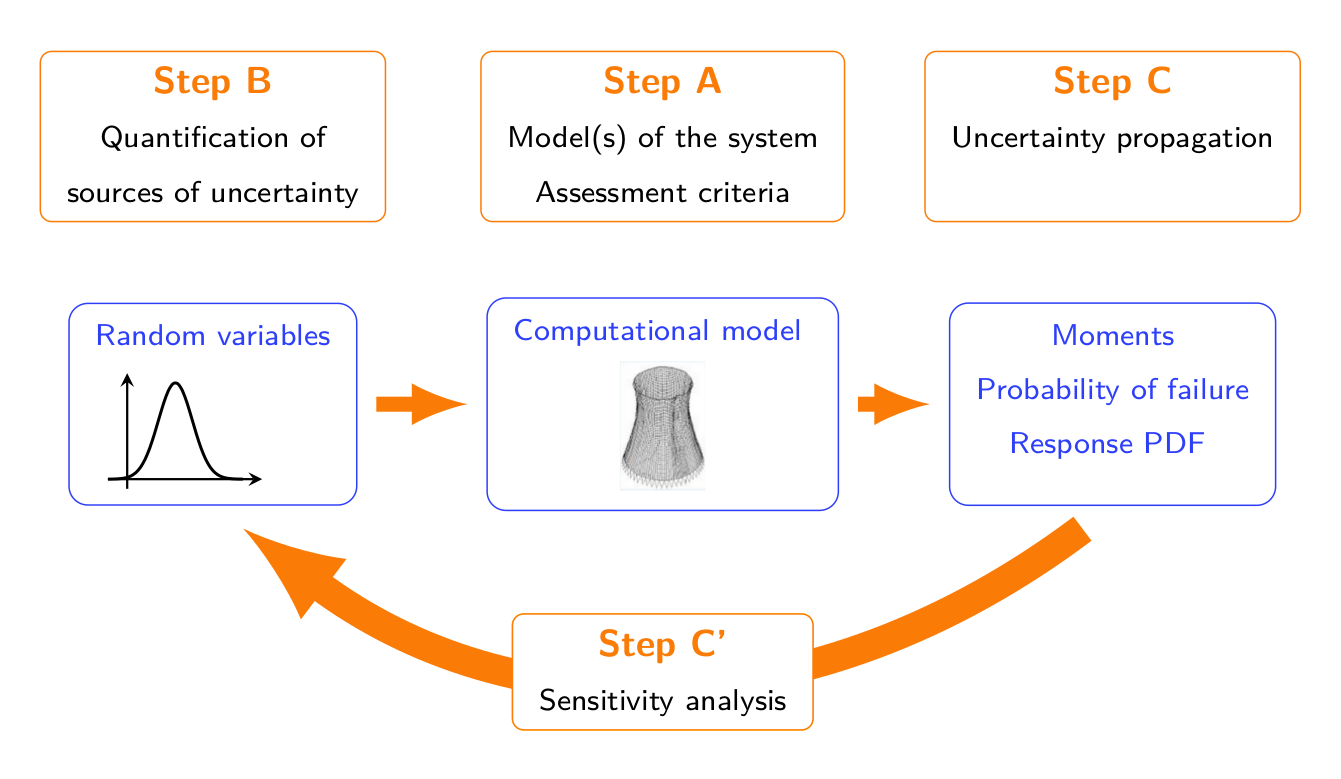
\includegraphics[width=0.8\textwidth]{img/background/UQ_steps.png}
    \caption{Uncertainty Quantification workflow. Taken from \href{http://www.uqlab.com/}{UQLab}.}
    \label{fig:uqlab_workflow}
\end{figure}

\subsection{Forward propagation or push-forward problem}\label{seq:forward}
Given the equation $\bm{Y}=\mathcal{M}(\bm{X})$ where: 
\begin{itemize}
\item $\bm{X} \in \mathcal{X} $ is a vector of  input parameters of the model,
\item $\mathcal{M}$ is a computational model, and
\item $\bm{Y} \in \mathcal{Y}$ is a vector that represents  quantities of interest (\textit{QoI}).
\end{itemize}
Suppose that the uncertainty about the inputs of $\mathcal{M}$ can be summarized in a probability distribution $P$ on $\mathcal{X}$. Then in a \textit{forward propagation}, the objective is to quantify the uncertainty of $\bm{Y}$, induced by $\bm{X}$ through $\mathcal{M}$.

The main objective of this thesis is a new method to quantify the uncertainty of the output of large-scale spatio-temporal models, that is a \textit{forward propagation problem}. In Section \ref{seq:methods_uq_propagation} some methods for \textit{forward propagation} are exposed; while in Section \ref{seq:uq_large_scale} we discuse about \textit{forward propagation} in large-scale spatio-temporal models.  

\subsection{Reliability or certification problem}\label{seq:reliability}
Suppose that some set $\mathcal{Y}_{fail}\subseteq \mathcal{Y}$ is identified as a 'failure set'. Then in a reliability analysis we are interesting in, given appropriate information about the input $X$ and a process $F$, determine the failure probability 
\begin{equation}
\mathcal{P}[\mathcal{M}(X)\in \mathcal{Y}_{fail}]
\end{equation}
Furthermore, how large will the deviation from acceptable performance be, and what are the consequences? \cite{Sullivan2015}

\subsection{Prediction problem}\label{seq:prediction}
Similar to the reliability problem, given a maximum acceptable probability error $\epsilon > 0$, find a set $\mathcal{Y}_{\epsilon}\subseteq \mathcal{Y}$ such that
\begin{equation}
\mathcal{P}[\mathcal{M}(X)\in \mathcal{Y}_{\epsilon}]\geq 1-\epsilon
\end{equation}

in other works, the prediction $\mathcal{M}(X)\in \mathcal{Y}_{\epsilon}$ is wrong with probability at most $\epsilon$.

\subsection{Inverse problem or parameter estimation}\label{seq:inverse}
Given some experimental measurements of the output $Y$ of the system and some computer simulation results from its mathematical model $\mathcal{M}$, inverse uncertainty quantification estimates the discrepancy between the experiment and the mathematical model (which is called \textit{bias correction}), and estimates the values of unknown parameters in the model if there are any (which is called \textit{parameter calibration}) \cite{GharibShirangi2014}. Generally this is a much more difficult problem than forward uncertainty propagation; however it is of great importance since it is typically implemented in a model updating process.

\subsection{Sensitivity Analysis}\label{seq:sensitivity}
Sensitivity analysis refers to the determination of the contributions of individual uncertain analysis inputs to the uncertainty in analysis results. The goal in sensitivity analysis is to apportion the uncertainty in $Y$ to the uncertainty in inputs $X$, \cite{Sankararaman2012}. 

\subsection{Model reduction or model calibration problem}\label{seq:calibration}
Construct another model $\mathcal{M}_{h}$ such that $\mathcal{M}_{h} \approx \mathcal{M}$ in an appropriate sense. 

\subsection{Model selection}
If, for the system $F$ we have a set of models $\mathcal{M} = \lbrace \mathcal{M}_{1}, \mathcal{M}_{2},...,\mathcal{M}_{n} \rbrace$, then a model selection problem consist in the selection of the most plausible model $\mathcal{M}_{i}$ that best fit the experimental data.

Sometimes a UQ problem consists of several of these problems coupled together, for example, one might have to solve an \textbf{\textit{inverse problem}} to produce or improve some model parameters, and then use those parameters to propagate some other uncertainties \textbf{\textit{forwards}}, and hence produce a \textbf{\textit{prediction}} that can be used for decision support in some \textbf{\textit{certification problem}} \cite{Sullivan2015}.

In this thesis we focus in \textbf{\textit{forward propagation problem}} although in chapter \ref{cap:use_cases} we introduce some queries that help to solve \textbf{\textit{reliability or certification}} and \textbf{\textit{prediction problem}}.

\section{Methods for Uncertainty Propagation}\label{seq:methods_uq_propagation}

\subsection{Sampling Methods}

\subsubsection{Monte Carlo}
To date, the MC simulation is the most powerful method for the uncertainty evaluation, \cite{Rajan2016a}.

Monte Carlo simulations (MCS) provide the most robust and straightforward way to
solve PDEs with random coefficients. In the case of (22.2), for instance, they consist
of (i) generating multiple realizations of the input parameters a and b, (ii) solving
deterministic PDEs for each realization, and (iii) evaluating ensemble statistics or
PDFs of these solutions. MCS do not impose limitations on statistical properties of
input parameters, entail no modifications of existing deterministic solvers, and are
ideal for parallel computing \cite{Higdon2017}.

\section{UQ in Large-scale Spatio-temporal models}\label{seq:uq_large_scale}
The emerging field of data science is largely lacking in generalizable methods for quantifying the uncertainty in the output of analysis systems. As a result, a major new research initiative needs to be initiated in this area. Since data science programs are just getting established in universities, this effort needs to be accompanied by relevant curriculum development \cite{Tobergte2013}

%The question of how to represent and communicate uncertainties is a topic of research both from a practical and theoretical point of view. A fair bit of theoretical research is aimed at the mathematical calculus of uncertainty. This includes extensions and alternatives to standard probabilistic reasoning, such as Dempster-Schafer theory and imprecise probabilities. When uncertainties are needed for investigations requiring computational models, additional considerations arise. For example, if the simulation output is a daily surface-temperature field over the globe for the next 200 years, representing uncertainty and dependencies is complex. Should ensembles be used to represent plausible outcomes? How should these ensembles of simulation output be stored? How can high-consequence/low-probability outcomes be discovered in this massive output? Here some research investigations attempt to leverage theory that exploits high dimensionality to bound probabilities and system behavior. Finally, even when uncertainties are well captured, how best to communicate such uncertainties to the public or to decision-makers is also a topic of ongoing research. 
%\cite{DEnergy2009}

\section{Software and Tools for UQ}
Currently, advances in uncertainty propagation and assessment have been paralleled by a growing number of software tools for uncertainty analysis, but none has gained recognition for a universal applicability, including case studies with spatial models and spatial model inputs. \cite{Sawicka2016}

These include both free software, like OpenTURNS (Andrianov et al., 2007), DACOTA (Adams et al., 2009) and DUE (Brown and Heuvelink, 2007), commercial, like COSSAN (Schuëller and Pradlwarter, 2006), or free, but written for a licenced software, e.g. SAFE (Pianosi et al., 2015) or UQLab (Marelli and Sudret, 2014) toolboxes for MATLAB. A broad review of existing software packages is available in Bastin et al. (2013). To the best of our knowledge, however, none of the existent software is specifically designed to be extended by the environmental science community. The use of powerful but complex languages like C++ (e.g. Dakota), Python (e.g. OpenTURNS) or Java (e.g. DUE) often discourages relevant portions of the non-highly-IT trained scientific community from the adoption of otherwise powerful tools.
spup-R package \cite{Sawicka2016}. De aqui saque lo de arriba tambien, aunque lo de arriba lo puedo buscar en sus respectivos papers y hablar un poco de cada uno de ellos.

\section{Summary}

\section{Concepts}
high-dimensional parameter spaces \cite{DEnergy2009}
computationally demanding forward models 
nonlinearity and/or complexity in the forward model

\section{Ideas a usar}
HPC and computational modeling play a dominant role in shaping the methodological developments and research in uncertainty qualification. Depending on the complexity of the uncertainty qualification investigation, anywhere from $10^{2}$ to $10^{8}$ runs of the computational model may be required. Thus, uncertainty qualification investigations may require extreme-computing environments (e.g., exascale) to obtain results in a useful time frame, even if a single run of the computational model does not require such resources. \cite{DEnergy2009}

Advances in computing over the past few decades—both in availability and power—have led to an explosion in computational models available for simulating a wide variety of complex physical (and social) systems. These complex models—which may involve millions of lines of code, and require extreme-computing resources—have led to numerous scientific discoveries and advances. This is because these models allow simulation of physical processes in environments and conditions that are difficult or even impossible to access experimentally. However, scientists’ abilities to quantify uncertainties in these model-based predictions lag well behind their abilities to produce these computational models. This is largely because such simulation-based scientific investigations present a set of challenges that is not present in traditional investigations.

\cite{DEnergy2009}

Until recently, the original approach of describing model parameters using single values has been retained, and consequently the majority of mathematical models in use today provide point predictions, with no associated uncertainty. \cite{Johnstone2015}

a 'typical' UQ problem involves one or more mathematical models for a process of interest, subject to some uncertainty about the correct form of, or parameter values for, those models. \cite{Sullivan2015}

Often, though not always, these uncertainties are treated probabilistically. \cite{Sullivan2015}

but how will you actually go about evaluating that expected value when it is an integral over a million-dimensional parameter space?
Practical problems from engineering and the sciences can easily have models with millions or billions of inputs
(degrees of freedom). \cite{Sullivan2015}

the language of probability theory is a powerful tool in describing uncertainty \cite{Sullivan2015}

“UQ studies all sources of error and uncertainty, including the following: systematic and stochastic measurement error; ignorance; limitations of theoretical models; limitations of numerical representations of those models; limitations of the accuracy and reliability of computations, approximations, and algorithms; and human error. A more precise definition is UQ is the end-to-end study of the reliability of scientific inferences.” \cite{DEnergy2009} (U.S. Department of Energy, 2009, p. 135)



In \cite{Sullivan2015} the authors remark that is important to appreciate both the underlying mathematics and the practicalities of implementation. In his work they focus in the presentation of the former and keep the latter in mind. In our work we do the opposite, we focus in the implementation keeping the math formalism in mind.

Probability theorists usually denote the sample space of a probability space by $\Omega$; PDE theorists often use the same letter to denote a domain in $\Re^{n}$ on which a partial differential equation is to be solved. In UQ, where the worlds of probability and PDE theory often collide, the possibility of confusion is clear. Therefore, this book will tend to use $\Theta$ for a probability space and \textbf{X} for a more general measurable space, which may happen to be the spatial domain for some PDE.

\chapter{Parallel Computation of PDFs on Large-scale Spatio-temporal Models}\label{cap:ji}

\begin{flushright}
	\textit{``...only assess the complete PDF allow aware decisions ''\\
	\cite{Lampasi2006}}
\end{flushright}

In the previous Chapter (\ref{cap:background}) we talk about the computational cost to compute the \textbf{PDF} on each spatio-temporal location of the output of a simulation, when we are in presence of a \textbf{LSSTM}. In the reviewed literature we don't find any work about how computational or time consuming could be this task. For this reason, in this Chapter we investigate the computational cost of trying to assess the \textbf{PDF} of those kinds of models.  

The rest of the Chapter is organized as follow: in Section \ref{sec:dataset} we present a dataset used in the experiments, Section \ref{sec:spark_architecture} present a distributed architecture over Spark to reduce the computational cost of the \textbf{PDF} fit. In Section \ref{sec:experiments} we discuss the results of the experiments, and finally in Section \ref{sec:summary} we summarize the results of this Chapter and discuss the disadvantage of the proposed approach.

\section{The Dataset}\label{sec:dataset}
To investigate the computational cost of trying to assess the \textbf{PDF} in \textbf{LSSTM} we use a various synthetic datasets. All the datasets are generate using the “HPC4E Seismic Test Suite”, a collection of four 3D models and sixteen associated tests that can be downloaded freely at the project's website (\url{https://hpc4e.eu/downloads/datasets-and-software}) \cite{deLaPuente2015}. Those models have been designed as a set of 16 layers with constant physical properties. The top layer delineates the topography and the other 15 delineate different layer interface surfaces or horizons. A Matlab script is provided that generates 3D gridded volumes and 2D gridded layer surfaces for any desired spacing and for three different variables $v_{p}(m/s)$, $v_{s}(m/s)$ and $density(Kg/m^3)$. For example, to generate a 3D volume with dimensions $250\times501\times501$ in the $v_{p}(m/s)$ variable we can use the values of Table \ref{tab:valuesOfVp}, and run the Matlab script \textit{generate-hpc4e-grid} . 

\begin{table}
\begin{center}
    \begin{tabular}{|l|l|}
    \hline
    \textbf{Layer} & $v_{p}(m/s)$ \\ \hline
    1     & 1618.92 \\ \hline
    2     & 1684.08 \\ \hline
    3     & 1994.35 \\ \hline
    4     & 2209.71 \\ \hline
    5     & 2305.55 \\ \hline
    6     & 2360.95 \\ \hline
    7     & 2381.95 \\ \hline
    8     & 2223.41 \\ \hline
    9     & 2712.06 \\ \hline
    10    & 2532.22 \\ \hline
    11    & 2841.03 \\ \hline
    12    & 3169.31 \\ \hline
    13    & 3252.35 \\ \hline
    14    & 3642.28 \\ \hline
    15    & 3659.22 \\ \hline
    16    & 4000.00 \\ \hline
    \end{tabular}
    \caption {Values of $v_{p}$ used in the generation of a single velocity field cube.}
    \label{tab:valuesOfVp}
    \end{center}
\end{table}

The first slice of this cube is shown in Figure \ref{fig:slice1}.

\begin{figure}[H]
    \centering
    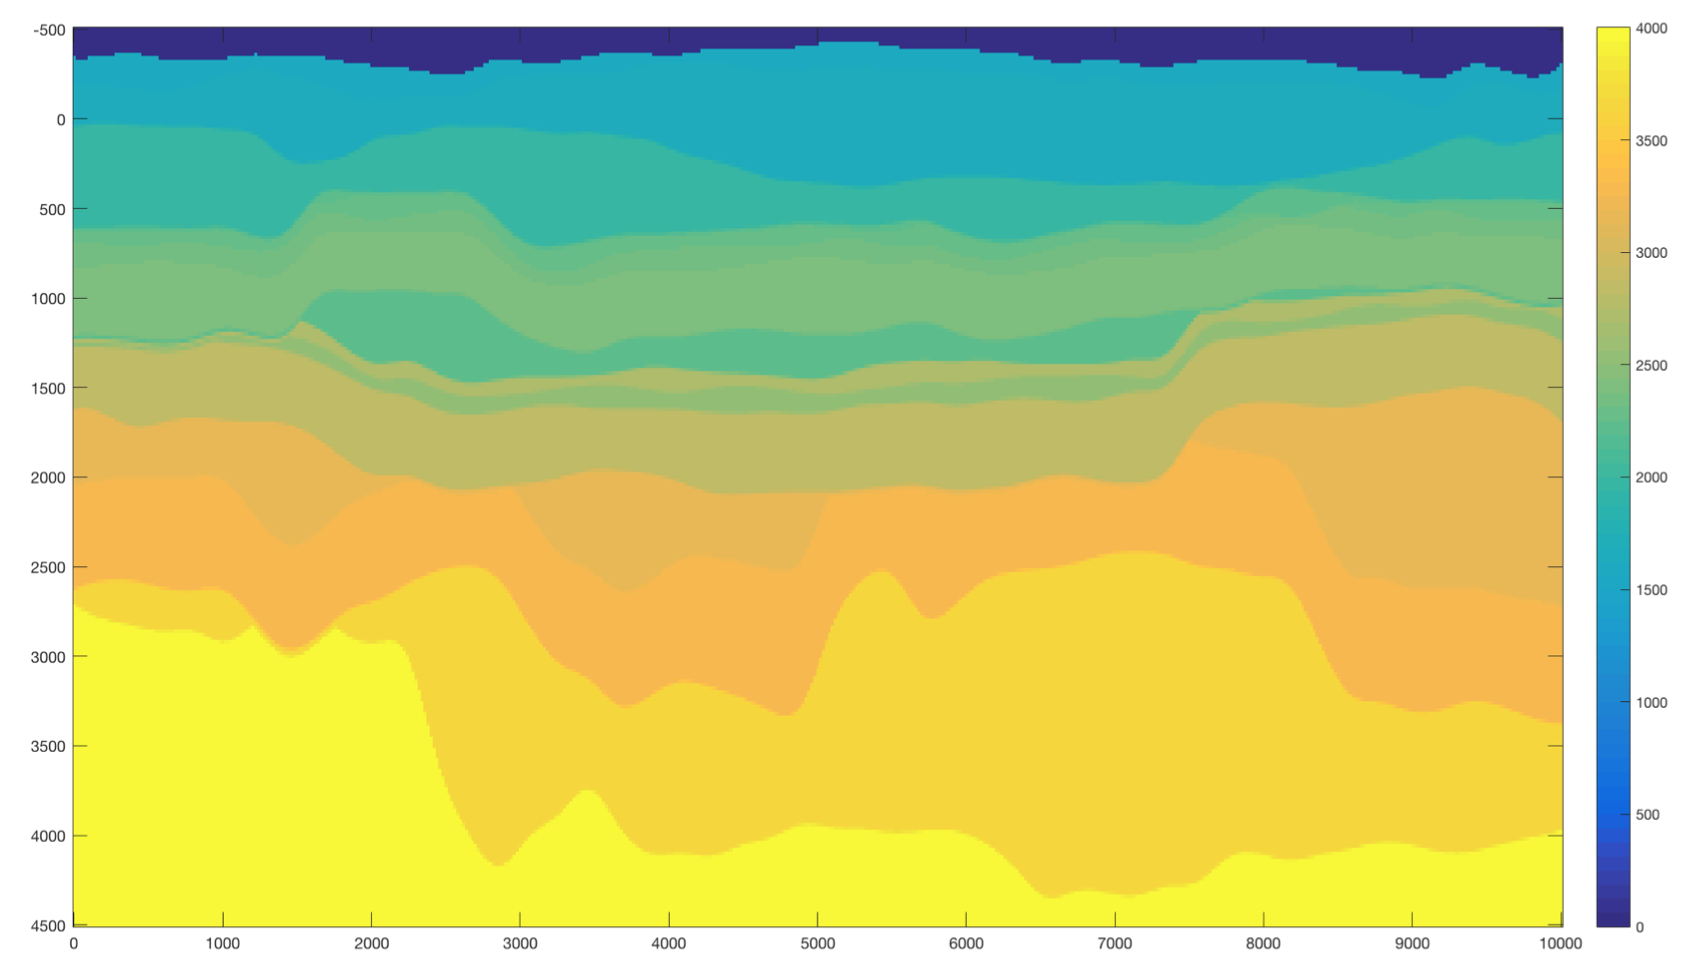
\includegraphics[width=0.8\textwidth]{images/velocity_field.png}
    \caption{One slice of the $250\times501\times501$ cube. In the slice we can distinguish between the different layers.}
    \label{fig:slice1}
\end{figure}

This script is to us as a mathematical model $v_{p}(x,y,z) = \mathcal{M}(v_{p})$ that receive $v_{p}$ as an input variable and generate a $v_{p}(x,y,z)$ as an output. In the benchmark the values of $v_{p}$ are fixed (Table \ref{tab:valuesOfVp}), so we cannot use it as is. We need to take the input, $v_{p}(m/s)$  in this case, as a random variable. To achieve this, we designate a \textit{PDFs} to each $v_{p}$ for each layer as shown in Table \ref{tab:PDFsOfVp}.

\begin{table}
\begin{center}
    \begin{tabular}{|l|l|l|}
    \hline
    \textbf{Layer} & \textbf{PDF Family}                & \textbf{Parameters}           \\ \hline
    1     & Gaussian & [1619, 711.2] \\ \hline
    2     & Gaussian & [3368, 711.2]               \\ \hline
    3     & Gaussian & [8839, 711.2]               \\ \hline
    4     & Gaussian & [7698, 301.5]               \\ \hline
    5     & Lognormal   & [7723, 294.7]               \\ \hline
    6     & Lognormal   & [7733, 292.2]               \\ \hline
    7     & Lognormal   & [7658, 312.1]               \\ \hline
    8     & Lognormal   & [3687, 368.7]               \\ \hline
    9     & Exponential & [3949, 394.9]             \\ \hline
    10   & Exponential & [5983, 711.2]               \\ \hline
    11   & Exponential & [3520, 352.0]              \\ \hline
    12   & Exponential & [3155, 315.5]              \\ \hline
    13   & Uniform     & [2541, 396.4]              \\ \hline
    14   & Uniform     & [2931, 435.3]              \\ \hline
    15   & Uniform     & [2948, 437.0]             \\ \hline
    16   & Uniform     & [3289, 471.1]              \\ \hline
    \end{tabular}
    \caption {PDFs and its parameters used to sampling the $v_{p}$, to generate n velocity models.}
    \label{tab:PDFsOfVp}
    \end{center}
\end{table}

Now, using a Monte Carlo method we can sampling the input variable $v_{p}$ and run as many simulations as we want using the model $v_{p}(x,y,z) = \mathcal{M}(v_{p})$, to posteriorly analyze the uncertainty in the output $v_{p}(x,y,z)$. An example of 1000 samplings of $v_{p}$ is shown in Figure \ref{fig:vp_1000_realizations}. Is clear that this is a not a real problem as a benchmark was not conceived as an uncertainty problem, but the datasets generated here are useful for our purposes.

\begin{figure}[ht]
    \centering
    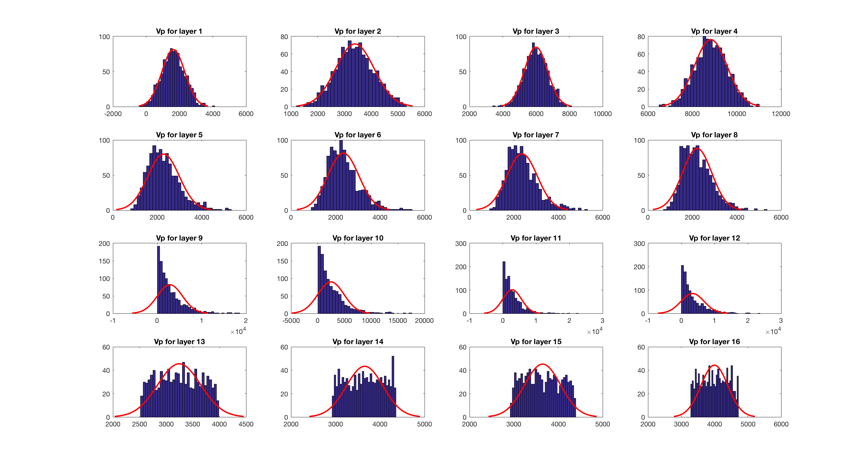
\includegraphics[width=0.8\textwidth]{images/vp_1000_realizations.png}
    \caption{Histograms of the 1000 samplings generated using Monte Carlo method and the PDFs reported in Table \ref{tab:PDFsOfVp}.}
    \label{fig:vp_1000_realizations}
\end{figure}

We generate three datasets, each one characterized by the dimensions $x \times y \times z$ of the cubes and the number of simulations. The datasets are name dataset1, dataset2 and dataset3, and its characteristics are summarized in Table \ref{tab:datasets}.

\begin{table}[H]
\centering
\begin{tabular}{c|c|c|c|}
\cline{2-4}
                               & dimensions                & simulations & size   \\ \hline
\multicolumn{1}{|c|}{dataset1} & $250\times501\times501$   & 1000        & 235 GB \\ \hline
\multicolumn{1}{|c|}{dataset2} & $501\times1001\times1001$ & 1000        & 1.9 TB \\ \hline
\multicolumn{1}{|c|}{dataset3} & $250\times501\times501$   & 10000       & 2.4 TB \\ \hline
\end{tabular}
\caption{Dimensions, number of simulations and size of the three datasets used to evaluate the computational cost of the \textbf{PDF} on a \textbf{LSSTM}.}
\label{tab:datasets}
\end{table}

\section{Architecture for Computing PDFs in Spark}\label{sec:spark_architecture}
We use two cluster testbeds, each with NFS, HDFS and Spark deployed. The first one, which we call LNCC cluster, is a cluster located at LNCC with 6 nodes, each having 32 CPU cores and 94 GB memory. The second one is a cluster of Grid5000, which we call G5k cluster, with 64 nodes, each having 16 CPU cores and 131 GB of RAM storage.

\section{Experimental Evaluation}\label{sec:experiments}

\section{Summary}\label{sec:summary}
The main conclusion of this Chapter is that compute a \textbf{PDF} on each spatio-temporal location is a computationally intensive task. The computational time can be reduced with 

\chapter[The Generalized Lambda Distribution]{The Generalized Lambda Distribution}\label{cap:gld}

\begin{flushright}
	\textit{``There are good reasons for using the GLD distribution \\
	methods... GLD fits have been used successfully in many fields ...\\
	Try the GLD first and stop there if the results are acceptable.''\\
	(Karian and Dudewicz, 2011)}
\end{flushright}


Fitting statistical distribution to data (real or simulated), is an important task in uncertainty quantification forward problem. When fitting data, one typically first selects a general class, or family, of distributions and then finds values for the distributional parameters that best match the observed data \cite{Lakhany2000}. One of this families is the Generalized Lambda Distribution (\textit{GLD}), originally proposed by Ramberg and Schmeiser in 1974, as a generalization of the Tukey's distribution (1947). The \textit{GLD} has tested 

In this chapter a review of the principal characteristics of the \textit{GLD}

it has been used in Monte Carlo simulations (Hogben, 1963), the modeling of empirical distributions (Okur, 1988; Ramberg et al., 1979), in response time modeling (Au-Yeung et al., 2004: Kumaran and Achary, 1996), supply chain (Ganesalinggam and Kumar, 2001) and in the sensitivity analysis of robust statistical methods (Shapiro et al., 1968).

\section{The Generalized Lambda Distribution}

The generalized lambda distribution is a continuous distribution defined in terms of it quantile function. Various parameterizations exist (see Section \ref{sec:gld_other_param}), but the most popular are the proposed by Ramberg and Schmeiser in 1974, Section \ref{sec:rs_gld}; and the proposed by Freimer et al. in 1988, Section \ref{sec:fmkl_gld}.

\subsection{The Ramberg and Schmeiser Parameterization}\label{sec:rs_gld}
The Generalized Lambda Distribution (\textit{GLD}) was proposed by Ramberg and Schmeiser in 1974 as an extention of the Tukey's distribution. It is represented by the quantil function:
\begin{equation}\label{eq:rs_param}
Q_{RS}(y|\lambda)=Q_{RS}(y|\lambda_{1}, \lambda_{2}, \lambda_{3}, \lambda_{4})=\lambda_{1}+\frac{y^{\lambda_{3}}-(1-y)^{\lambda_{4}}}{\lambda_{2}}
\end{equation}
where $Q_{RS}=F^{-1}$ is the quantile function for probabilities $y$, wiht $y\in[0,1]$; $\lambda_{1}$ and $\lambda_{2}$ are the location and scale parameteres, and $\lambda_{3}$ and $\lambda_{4}$ determine the skewness and kurtosis of the $GLD(\lambda_{1}, \lambda_{2}, \lambda_{3}, \lambda_{4})$.

The probability density function of the \textit{GLD} at the point $x=Q_{RS}(y)$ is given by:
\begin{equation}\label{eq:rs_pdf}
f(x)=f(Q_{RS}(y))=\frac{\lambda_{2}}{\lambda_{3}y^{\lambda_{3}-1}+\lambda_{4}(1-y)^{\lambda_{4}-1}}
\end{equation}

In order to have a valid distribution function, the probability density function $f(x)$ need to be positive for all $x$ and integrates to one over the allowed domain:
\begin{equation}
f(x) \geqslant 0
\end{equation}
\begin{equation}
\int f(x)dx=1
\end{equation}

This impose complex constraints on the parameters and support regions of the \textit{RS} parameterization, as summarized in table \ref{tab:rs_conts} and figure \ref{fig:rs_regions}.

% Please add the following required packages to your document preamble:
% \usepackage{multirow}
\begin{table}[]
\centering
\caption{Support regions of the GLD and conditions on the parameters given by the RS parameterization to define a valid distribution function \cite{Karian2011}. The support regions are displayed in Fig. \ref{fig:rs_regions}. Note that there are no conditions on $\lambda_{1}$ to obtain a valid distribution.}
\label{tab:rs_conts}
\begin{tabular}{c|c|c|c|c|c}
\hline
Region             & $\lambda_{2}$         & $\lambda_{3}$      & $\lambda_{4}$      & Q(0)                                                 & Q(1)                                                 \\ \hline
\multirow{3}{*}{1} & \multirow{3}{*}{$<0$} & $<=-1$             & $>=1$              & \multirow{3}{*}{$-\infty$}                           & \multirow{3}{*}{$\lambda_{1}+\frac{1}{\lambda_{2}}$} \\
                   &                       & $-1<\lambda_{3}<0$ & $>1$               &                                                      &                                                      \\
                   &                       & \multicolumn{2}{c|}{$\frac{(1-\lambda_{3})^{1-\lambda_{3}}(\lambda_{4}-1)^{\lambda_{4}-1}}{(\lambda_{4}-\lambda_{3})^{\lambda_{4}-\lambda_{3}}}=\frac{-\lambda_{3}}{\lambda_{3}}$}            &                                                      &                                                      \\ \hline
\multirow{3}{*}{2} & \multirow{3}{*}{$<0$} & $>=1$              & $<=-1$             & \multirow{3}{*}{$\lambda_{1}-\frac{1}{\lambda_{2}}$} &                                                      \\
                   &                       & $>1$               & $-1<\lambda_{4}<0$ &                                                      & $\infty$                                             \\
                   &                       & \multicolumn{2}{c|}{$\frac{(1-\lambda_{4})^{1-\lambda_{4}}(\lambda_{3}-1)^{\lambda_{3}-1}}{(\lambda_{3}-\lambda_{4})^{\lambda_{3}-\lambda_{4}}}=\frac{-\lambda_{4}}{\lambda_{3}}$}            &                                                      &                                                      \\ \hline
\multirow{3}{*}{3} & \multirow{3}{*}{$>0$} & $>0$               & $>0$               & $\lambda_{1}-\frac{1}{\lambda_{2}}$                  & $\lambda_{1}+\frac{1}{\lambda_{2}}$                  \\
                   &                       & $=0$               & $>0$               & $\lambda_{1}$                                        & $\lambda_{1}+\frac{1}{\lambda_{2}}$                  \\
                   &                       & $>0$               & $=0$               & $\lambda_{1}-\frac{1}{\lambda_{2}}$                  & $\lambda_{1}$                                        \\ \hline
\multirow{3}{*}{4} & \multirow{3}{*}{$<0$} & $<0$               & $<0$               & $-\infty$                                            & $\infty$                                             \\
                   &                       & $=0$               & $<0$               & $\lambda_{1}$                                        & $\infty$                                             \\
                   &                       & $<0$               & $=0$               & $-\infty$                                            & $\lambda_{1}$                                        \\ \hline
\end{tabular}
\end{table}

\begin{figure}[H]
    \centering
    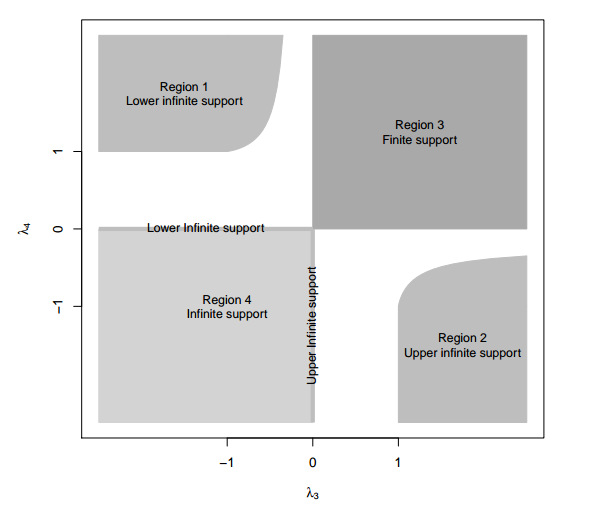
\includegraphics[width=0.8\textwidth]{img/gld/rs_regions.png}
    \caption{Support regions of the GLD in the RS parameterization that produce valid statistical
distributions.}
    \label{fig:rs_regions}
\end{figure}

\subsection{The FMKL Parameterization}\label{sec:fmkl_gld}
To circumvent the constraints on the \textit{RS} parameter values, Freimer et al. \cite{Freimer1988} introduced a new parameterization called \textit{FKML}, equation \ref{eq:fmkl_param}.

\begin{equation}\label{eq:fmkl_param}
Q_{FMKL}(y|\lambda_{1}, \lambda_{2}, \lambda_{3}, \lambda_{4})=\lambda_{1}+\frac{1}{\lambda_{2}}\left[\frac{y^{\lambda_{3}}-1}{\lambda_{3}} - \frac{(1-y)^{\lambda_{4}}-1}{\lambda_{4}} \right] 
\end{equation}

As in the previous parameterization, $\lambda_{1}$ and $\lambda_{2}$ are the location and scale parameters, but in this one $\lambda_{3}$ and $\lambda_{4}$ are the tail index parameters. The advantage over the previous parameterization is that the only constraint on the parameters is that $\lambda_{2}$ must be positive. Figure \ref{fig:fmkl_regions} displays the support regions of the \textit{GLD} in the \textit{FKML} parameterization, table \ref{tab:fmkl_conts}.

\begin{table}[]
\centering
\caption{Support regions of the \textit{GLD} given by the \textit{FMKL} parameterization \cite{Marcondes2018}.}
\label{tab:fmkl_conts}
\begin{tabular}{c|c|c|c}
\hline
$\lambda_{3}$ & $\lambda_{4}$ & Q(0)                                           & Q(1)                                           \\ \hline
$>0$          & $>0$          & $\lambda_{1}-\frac{1}{\lambda_{2}\lambda_{3}}$ & $\lambda_{1}+\frac{1}{\lambda_{2}\lambda_{4}}$ \\ \hline
$>0$          & $\leq0$         & $\lambda_{1}-\frac{1}{\lambda_{2}\lambda_{3}}$ & $\infty$                                       \\ \hline
$\leq0$         & $>0$          & $-\infty$                                      & $\lambda_{1}+\frac{1}{\lambda_{2}\lambda_{4}}$ \\ \hline
$\leq0$         & $\leq0$         & $-\infty$                                      & $\infty$                                       \\ \hline
\end{tabular}
\end{table}

\begin{figure}[H]
    \centering
    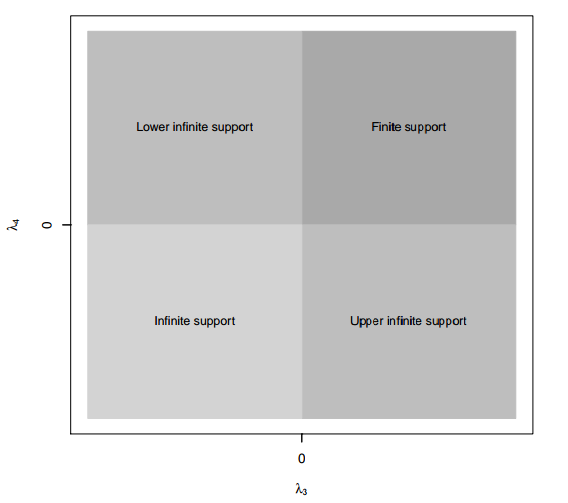
\includegraphics[width=0.8\textwidth]{img/gld/fmkl_regions.png}
    \caption{Support regions of the \textit{GLD} in the \textit{FMKL} parameterization that produce valid statistical
distributions.}
    \label{fig:fmkl_regions}
\end{figure}

The probability density function of the \textit{FMKL}-\textit{GLD} at the point $x=Q_{FMKL}(y)$ is given by \cite{Su2015}:
\begin{equation}\label{eq:fmkl_pdf}
f(x)=f(Q_{FMKL}(y))=\frac{\lambda_{2}}{y^{\lambda_{3}-1}+(1-y)^{\lambda_{4}-1}}
\end{equation}

Although both the \textit{RS} and \textit{FMKL} \textit{GLD} are generalizations of Tuckey's Lambda Distribution, they are not equivalent, so that the distribution fitted by one parametrization to a dataset differs in general from the one fitted by the other \cite{Marcondes2018}. Both of these representations can present a wide variety of shapes and therefore are utilized in practice; however, it is generally the \textit{FMKL GLD} preferred due to the ease in its use \cite{Corlu2016}. In this thesis, we also use the \textit{FMKL GLD} representation.

\subsection{Other Parameterizations}\label{sec:gld_other_param}
One of the criticisms of the \textit{GLD} is that its skewness is expressed in terms of both tail indices $\lambda_{3}$ and $\lambda_{4}$. In one approach addressing this concern, a five-parameter \textit{GLD} was introduced by Joiner et al. \cite{Joiner1971}, which, expressed in the \textit{FKML} parameterization, can be written as,
\begin{equation}\label{eq:jr_param}
Q_{JR}(y|\lambda_{1}, \lambda_{2}, \lambda_{3}, \lambda_{4})=\lambda_{1}+\frac{1}{2 \lambda_{2}}\left[(1-\lambda_{5})\frac{y^{\lambda_{3}}-1}{\lambda_{3}} - (1+\lambda_{5})\frac{(1-y)^{\lambda_{4}}-1}{\lambda_{4}} \right] 
\end{equation}

It has $\lambda_{1}$ and $\lambda_{2}$ as the location and scale parameters, and an asymmetry parameter, $\lambda_{5}$, which weights each side of the distribution and the two tail indices, $\lambda_{3}$ and $\lambda_{4}$. The conditions on the parameters are $\lambda_{2} > 0$ and $-1 < \lambda_{5} < 1$. The drawback of this parameterization is that the additional parameter can make the estimation of the parameter values even more difficult.

In \cite{Chalabi2012} the authors introduce a new parameterization of the \textit{GLD} that transform the \textit{FMKL} parameterization, equation \ref{eq:fmkl_param} in terms of an asymmetry and steepness parameter without adding a new variable. Its major advantage is that provides an intuitive interpretation of its parameters. A new \textbf{R} package called \textbf{gldist} was implemented with the new \textit{GLD} parameterization, along with the parameter estimation methods they present in his work. The problem with this parameterization is  that the \textbf{R} package was removed from the official repository because of the code is out of date.

\section{FMKL GLD Shapes}\label{sec:gld_shapes}
Both \textit{RS} and \textit{FMKL} \textit{GLD} can describe a variety of shapes, examples: U-shaped, bell shaped, triangular, and exponentially \cite{Su2007}. At the same time they also provide good fits to many well know distributions. In the case of \textit{RS GLD} and extensive study can be found in \cite{Karian2011}, for the \textit{FMKL GLD} see \cite{Freimer1988}. 

Those properties of the \textit{GLD} are important to our purpose for two reasons: first we don't need previous knowledge to use the \textit{GLD} to fit any dataset, that is exactly the case in large-scale spatio-temporal models, and second the \textit{GLD} can be compared and grouped based on its shapes, that allow us to answer the \textbf{RQ1} as we show in Chapter \ref{cap:gld_clustering}.

As the \textit{FMKL GLD} parameterization is the one selected to be used in this thesis, in the next sub-sections we present a brief review of its shapes and how this parameterization fit some well-known distributions.

The shape of the \textit{GLD} are dependent of its $\lambda$ values. In the case of the \textit{FMKL GLD} parameterization, Freimer et al. \cite{Freimer1988} classify the shapes into five categories depending on the variety of distributions that can be represented by the several combinations of the shape parameters $\lambda_{3}$ and $\lambda_{4}$. In particular, Class-I ($\lambda_{3} < 1$, $\lambda_{4}<1$) represents unimodal densities with continuous tails. This class is subdivided in $I_{a}$ $(\lambda_{3}, \lambda_{4} \leq 1/2)$, $I_{b}$ $(1/2 < \lambda_{3} < 1, \lambda_{4} \leq 1/2)$ and $I_{c}$ $(1/2 < \lambda_{3} < 1, 1/2 < \lambda_{4} < 1)$. In $I_{a}$ we find distributions such us $Gaussian (Normal)$, $Beta(2.3)$ and $\Gamma(\alpha = 5)$; in $I_{b}$ $\Gamma(\alpha = 3)$ and $Lognormal(\sigma=0.5)$; and in $I_{c}$ distributions as the example of Class-I in Figure \ref{fig:fmkl_classes}.  

Class-II ($\lambda_{3}>1$, $\lambda_{4}<1$) represents monotone pdfs similar to the $Exponential$ distribution, $Beta(1.2)$ or $Lognormal(\sigma=1.0)$. Class-III ($1<\lambda_{3}<2$, $1<\lambda_{4}<2$) represents U-shaped densities with truncated tails, Class-IV ($\lambda_{3}>2$, $1<\lambda_{4}<2$) represents S-shaped densities, and Class-V ($\lambda_{3}>2$, $\lambda_{4}>2$) represents unimodal densities with truncated tails. Figure \ref{fig:fmkl_classes} provides the shapes that are represented by the parameters indicated in Table \ref{tab:fmkl_classes}.

\begin{table}[H]
\centering
\caption{Examples of the five categories of distributions the \textit{FMKL GLD} can represent.}
\label{tab:fmkl_classes}
\begin{tabular}{lllll}
\hline
          & $\lambda_{1}$ & $\lambda_{2}$ & $\lambda_{3}$ & $\lambda_{4}$ \\ \hline
Class-I   & 0             & 1             & 0.5           & 0.6           \\
Class-II  & 0             & 1             & 2             & 0.5           \\
Class-III & 0             & 1             & 1.5           & 1.5           \\
Class-IV  & 0             & 1             & 2.5           & 1.5           \\
Class-V   & 0             & 1             & 3             & 3             \\ \hline
\end{tabular}
\end{table}

\begin{figure}[H]
    \centering
    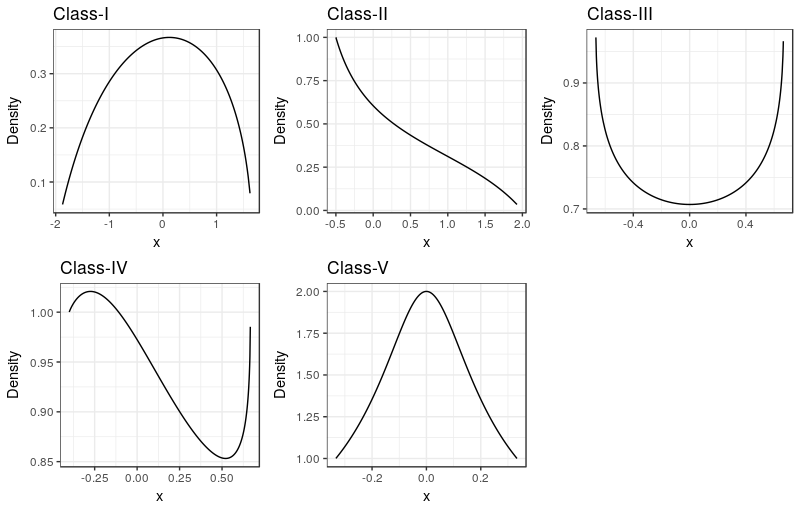
\includegraphics[width=0.8\textwidth]{img/gld/fmkl_classes.png}
    \caption{Examples of the five categories of shapes the \textit{FMKL GLD} can represent.}
    \label{fig:fmkl_classes}
\end{figure}

Figure \ref{fig:fmkl_classes_l3_l4} show the five categories of the \textit{FMKL GLD} shapes in $(\lambda_{3}, \lambda_{4})$ space. There are two regions in this figure that were left out of the analysis, the regions with ($\lambda_{3}<1$, $\lambda_{4}>1$) and ($1<\lambda_{3}<2$, $\lambda_{4}>2$). Those regions are symmetric to region II and IV respectively, see Figure \ref{fig:symmetry}.

\begin{figure}[H]
    \centering
    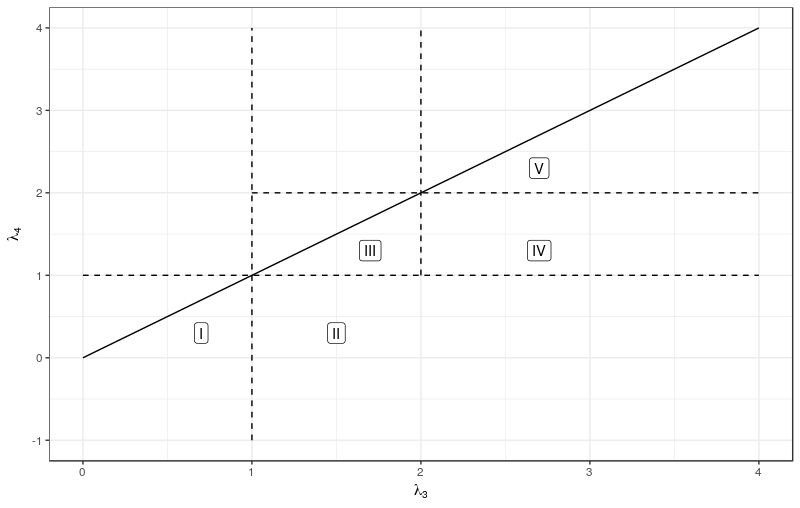
\includegraphics[width=0.8\textwidth]{img/gld/classes_l3_l4.png}
    \caption{The five categories of shapes of the \textit{FMKL GLD} in the $(\lambda_{3}, \lambda_{4})$ space.}
    \label{fig:fmkl_classes_l3_l4}
\end{figure}

\begin{figure}[H]
    \centering
    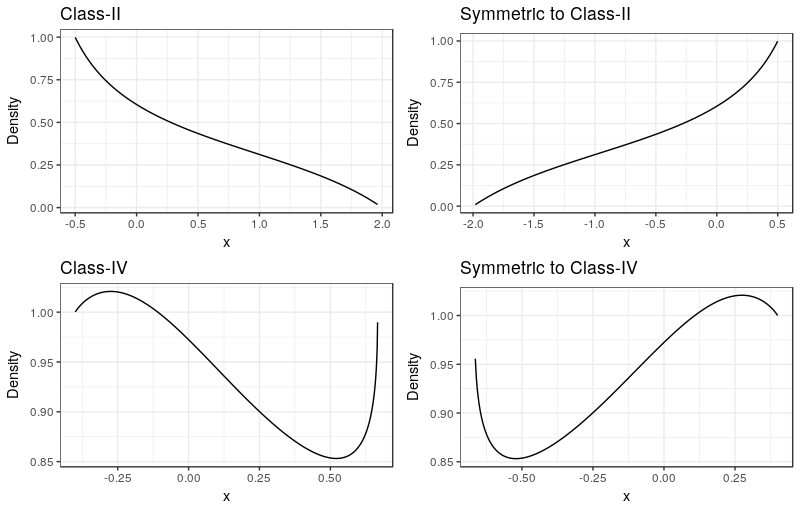
\includegraphics[width=0.8\textwidth]{img/gld/symetrics.png}
    \caption{Symmetry of the regions ($\lambda_{3}<1$, $\lambda_{4}>1$) and ($1<\lambda_{3}<2$, $\lambda_{4}>2$) with respect to  region II and IV.}
    \label{fig:symmetry}
\end{figure}

The results presented in this section are extremely important to our approach because they are the bases of the clustering algorithms we propose in Chapter \ref{cap:gld_clustering}.


\section{Numerical Methods to Fit the GLD to Data}\label{sec:gld_numerical_methods}
Given a random sample $x_{1},x_{2},x_{3},...x_{n}$, the basic problem in fitting a statistical distribution to this data is that of approximating the distribution from which the sample was obtained. If it is known, because of theoretical considerations, that the distribution is of a certain type (e.g., a gamma distribution with unknown parameters), then through moment matching, or some other means, one can determine a specific distribution that fits the data. This, however, is generally not the case and, in the absence of any knowledge regarding the distribution, it makes sense to appeal to a flexible family of distributions and choose a specific member of that family \cite{Karian2011}.

There are two different parameter estimation philosophies, \textbf{direct estimation methods}, such as least-squares estimation with order statistics [Ozturk and Dale, 1985] and with percentiles [Karian and Dudewicz, 1999, 2000; Fournier et al., 2007; King and MacGillivray, 2007; Karian and Dudewicz, 2003]; the methods of moments [Ozturk and Dale, 1982; Gilchrist, 2000], L-moments [Gilchrist, 2000; Karvanen and Nuutinen, 2008], and trimmed L-moments [Asquith, 2007]; and the goodness-of-fit method with histograms \cite{Su2005} and with maximum likelihood estimation \cite{Su2007}. On the other side, \textbf{stochastic methods} have been introduced with various estimators such as goodness-of-fit [Lakhany and Mausser, 2000] or the starship method [King and MacGillivray, 1999]. 

Moreover, \cite{Lampasi2006}

Numerical maximum log likelihood estimation for generalized lambda distributions 

\cite{Lodziensis2013}
\cite{Lakhany2000}
\cite{Fournier2007}
\cite{Marcondes2018}
Review and Genetic Algorithms approach \cite{Corlu2016}

\section{GLD Approximations of Some Well-Known Distributions}\label{sec:gld_fit_other}
For the $GLD(\lambda_{1}, \lambda_{2}, \lambda_{3}, \lambda_{4})$ to be useful for fitting distributions to data, it should be able to provide good fits to many of the distributions the data may come from. In \cite{Karian2011}, the authors explore how the \textit{GLD} fit sixteen well-known distributions using the \textit{RS GLD} parameterization. Here we explore how the \textit{GLD} fit eight distributions, but using the \textit{FMKL} parameterization.

In Table \ref{tab:gld_fit_other} we show the original distribution, the four $\lambda$ values of the fit and the result of apply a Kolmogorov-Smirnov test to validate the good of the fit.

\begin{table}[H]
\centering
\caption{GLD Approximations of 8 Well-Known Distributions}
\label{tab:gld_fit_other}
\begin{tabular}{l|l|l|l|l|l|l}
\hline
Distribution & Parameters                    & $\lambda_{1}$ & $\lambda_{2}$ & $\lambda_{3}$ & $\lambda_{4}$ & KS-test \\ \hline
Normal       & $\textsc{N}(0, 1)$                     & -0.04263   & 1.49039    & 0.13787    & 0.12571    & 951     \\ \hline
Uniform      & $U(0, 1)$                     & 0.46250     & 2.16223     & 1.00008     & 0.8614     & 912     \\ \hline
Exponential  & $\theta = 1$                  & 0.49150     & 1.40546     & 1.44813     & -0.10419    & 923     \\ \hline
Chi-Square   & $nu = 5$                      & 4.141853    & 0.486702    & 0.508298    & -0.045440   & 911     \\ \hline
Gamma        & $(\alpha = 5, \theta = 3)$    & 1.535078    & 1.846312    & 0.410183    & 0.027492    & 885     \\ \hline
Weibull      & $(\alpha = 1, \beta = 5)$     & 2.684657    & 0.263865    & 1.413826    & -0.067658   & 940     \\ \hline
Lognormal    & $(\mu = 0, \sigma = 1/3)$     & 0.984696    & 4.516254    & 0.324879    & -0.074348   & 903     \\ \hline
Beta         & $(\beta_{3} = \beta_{4} = 1)$ & 0.50092     & 2.00702     & 0.99505     & 1.00060     & 906     \\ \hline
\end{tabular}
\end{table}

As was expected the results are slightly different to those presented by Karian et al., as we use other parameterization. The KS-test value was over 900 in seven cases and near 900 in the case of the Gamma distribution. This result suggests us that the fit was good. All the fit provides $(\lambda_{3}, \lambda_{4})$ values that match the shape region each distribution belongs to.


\section{Fitting Mixture Distributions Using a Mixture of Generalized Lambda Distributions}\label{sec:gld_mixture}
Esto esta en \cite{Tobergte2013}

Maximum Log Likelihood Estimation using EM Algorithm and Partition Maximum Log Likelihood Estimation for Mixtures of Generalized Lambda Distributions  \cite{Su2011}. En este articulo presenta ejemplos bien extraños.

Fitting the GLD and compare with the normal mixture \cite{Ning2008}

\section{GLD Random Variate Generation}\label{sec:gld_random_variate}
An important thing to take into account when we substitute the raw data produced as an output of a simulation process, by its \textit{PDF} is that those \textit{PDFs} need to allow us to reproduce the original data as close as possible. The outcome produced by a particular \textit{PDF} is known as random variate, its definition is:

\begin{defn} 
A \textbf{random variate} is a particular outcome of a random variable. The random variates which are other outcomes of the same random variable might have different values.
\end{defn}

Random variates are used when simulating processes driven by random influences. One of the important applications of the \textit{GLD} has been the generation of random variables for Monte Carlo studies \cite{Mustafa2016}.

This fact is justified by the following theorem, enunciated by Karian and Dudewicz (2010).

\begin{thm}
If $Q_{X}(y)$ is the percentile function of a random variable $X$, and $U$ is a uniform random variable
on $(0, 1)$ then $Q_{X}(U)$ has the same \textit{PDF} as does $X$.
\end{thm}

For a proof, also see p. 156 of Karian and Dudewicz (1999). The percentile function is not available in a closed (or easy-to-work-with) form for many of the most important distributions, such as the normal distribution. However, the GLD is (see sections \ref{sub:rs_gld} and \ref{sub:fmkl_gld}) defined by its p.f., which is a simple-to-calculate expression.

Thus, \textbf{r.v.s for a simulation study can easily be generated from any distribution that can be modeled by a GLD.}

\begin{exmp}
Suppose we have modeled an important \textbf{r.v.} by an approximate standard normal distribution $X$. We show in Section \ref{sec:gld_fit_other} that a close fit to the standard normal is available via the \textit{RS-GLD} with 
\begin{equation}
(\lambda_{1}, \lambda_{2}, \lambda_{3}, \lambda_{4}) = (0, 0.1975, 0.1349, 0.1349)
\end{equation}
and this \textit{GLD} has \textbf{p.f.} 
\begin{equation}
Q(y) = \frac{y^{0.1349}-(1-y)^{0.1349}}{0.1975}
\end{equation}
\end{exmp}

Thus, if $U_{1}, U_{2},...$ are independent uniform \textbf{r.v.s} on $(0, 1)$, then 
\begin{equation}\label{eq:random_variate}
Q(U_{1}), Q(U_{2}),...
\end{equation}
are independent and (approximately) $N(0, 1)$ \textbf{r.v.s} for the simulation study at hand.

This theorem means that, independently of the nature of the dataset (Normal, Exponential, etc.), when we fit a GLD to it, we can proceed similarly to the example above. That is, we just need to generate a stream of independent uniform \textbf{r.v.s} on $(0, 1)$, and then evaluate the equation \ref{eq:random_variate}. There are a number of good sources of independent uniform r.v.s on $(0, 1)$ \cite{Karian2011}. 

This is an important property of the \textit{GLD} that allow us to substitute the raw data by the four lambdas of the \textit{GLD} that best fit it (if the fit is a good one), with the warranty that if we need to go back, the \textit{GLD} could generate a good representation of the original data.

It is evident that the \textit{GLD} allows easy generation of random variables from every kind of distribution, because featuring an explicit and accessible $Q_{X}(y)$ reduces it to a uniform generation in $[0,1]$, \cite{Lampasi2006}.


\section{GLD and Uncertainty Quantification}
\subsection{Related Works}
A solution to determining the reliability of products Using Generalized Lambda Distribution \cite{Movahedi2013}

Fundamental Reference \cite{Lampasi2006}

\cite{Cox2012}

\subsection{Relevance of GLD in Uncertainty Quantification}
The use of the \textit{GLD} to quantify the uncertainty is justified because: 
\begin{itemize}
\item the \textit{GLD} fits the \textit{PDF} of a wide variety of datasets, including those that follow distributions such as normal, uniform, Student's t, U-shaped, exponential, etc;
\item no prior knowledge is needed to fit the \textit{GLD} to a dataset, which is practical and suitable for automatic and software procedures;
\item the \textit{PDF} is completely characterized by the four parameters of the \textit{GLD}, which represents a reduction in the amount of data that must be stored for post-processing;
\item the shape of the \textit{GLD} is governed by its parameters, so the \textit{GLDs} can be grouped  based on their shapes, which is especially useful for further queries; and
\item in cases where mixture of distributions are needed, \textit{GLD} mixtures could be a very good option;
\item a \textit{GLD} is good for random variate generation.
\end{itemize}
\cite{Ning2008} 

\section{The GLDEX R package}\label{sec:gldex}
In the implementation of our approach, we use the \textbf{\textit{GLDEX}}\footnote{https://cran.r-project.org/web/packages/GLDEX/index.html} \textbf{\textit{R}} package \cite{Su2007}. The GLDEX R package provides fitting algorithms with two objectives: (i) to provide a smoothing device to fit distributions to data using the weight and unweighted discretised approach based on the bin width of the histogram; (ii)  to provide a definitive fit to the data set using the maximum likelihood estimation.

The GLDEX package also provides diagnostic tests to examine the quality of fit through the resample Kolmogorov-Smirnoff test, quantile plots and comparison of the mean, variance, skewness and kurtosis between the empirical data and the fitted distribution.

The GLDEX package is used in this thesis to: (i) fit the \textit{GLD} distribution to a dataset on each spatio-temporal location; (ii) examine the quality of the fit; (iii) sampling any spatio-temporal location based on its \textit{GLD}.

\section{Conclusions}


\chapter{Our Approach}\label{our_approach}

\section{Fit the spatio-temporal dataset to the GLD}

Aqui tengo que poner:
\begin{itemize}
\item Fit each spatio-temporal point to a corresponding GLD.
\item Evaluate if the resulting GLD is valid on each spatio-temporal location.
\item Perform a ks-test to evaluate if the quality of the fit on each spatio-temporal location.
\end{itemize}

\section{Clusterizing the GLD based in its lambda values}

\section{Use of GLD mixture to characterize the uncertainty in an spatio-temporal region}

\section{Information entropy as a measure of the uncertainty in an spatio-temporal region}

\section{Information entropy and model selection}

\section{Conclusions}
\chapter[Clustering Uncertain Data Based on GLD Similarity]{Clustering Uncertain Data Based on GLD Similarity}\label{cap:gld_clustering}

In Chapter \ref{cap:gld} we exposed the two most important parameterizations of the \textit{GLD} and select the \textit{FMKL} as  the one to be used for the rest of the  thesis. In this parameterization $\lambda_{1}$ represent the location of the \textit{GLD} and is directly related to the mean of the distribution. $\lambda_{2}$ is the scale, directly related to the standard deviation; and $\lambda_{3}$ and $\lambda_{4}$ represent the left and right tails of the distribution. Combinations of $\lambda_{3}$ and $\lambda_{4}$ can be used to estimate the skewness and kurtosis of the distribution.

As $\lambda_{2}$ define the dispersion, and $\lambda_{3}$ and $\lambda_{4}$ the shape of a \textit{GLD}, so the combination of those parameters are the responsible of the quantification of the uncertainty, from the \textit{GLD} point of view.

The \textbf{RQ.1} we formulate in the Introduction (see Chapter \ref{cap:intro}) is:

\begin{tcolorbox}
\textbf{RQ1.} how to group the output of the UQ process based on the similarity of the uncertainty?
\end{tcolorbox}

If the uncertainty in a \textit{GLD} is characterized by $\lambda_{2}$, $\lambda_{3}$ and $\lambda_{4}$ and we are interesting into group the uncertainty based on the similarity, is clear that we need to explore how to group the \textit{GLDs} based on its $\lambda$ values. This is the main objective of this Chapter, that is organized as follow: in Section \ref{sec:related_works} a brief review of some related works is performed, and the advantage and drawbacks of those works are highlighted. Some considerations about the possibilities of the use of the \textit{GLD} to solve some of the drawbacks are commented. Next, in section \ref{sec:clustering_gld} our hypothesis about the use of the \textit{GLD} to clustering uncertain data, is presented. Sections \ref{sec:synthetic_I} and \ref{sec:synthetic_II} present two synthetics datasets and the results of the clustering technique. Those results help us to validate our hypothesis. Finally, section \ref{sec:clustering_summary} summarize and discuss the main results of the Chapter.

 \section{Related Works}\label{sec:related_works}

\cite{Jiang2011}

\section{Clustering Based on GLD}\label{sec:clustering_gld}

According to Lampasi et al. \cite{Lampasi2006}, a particular $GLD(\lambda_{1},\lambda_{2},\lambda_{3},\lambda_{4})$ can be rewrite as: 

\begin{equation}\label{eq:rewrite_gld}
GLD(\lambda_{1},\lambda_{2},\lambda_{3},\lambda_{4}) = \lambda_{1} + \frac{1}{\lambda_{2}}GLD(0,1,\lambda_{3},\lambda_{4}) 
\end{equation}

Based on the second term of Equation \ref{eq:rewrite_gld}, our hypothesis is that we can group the uncertainty using clustering algorithms above $\lambda_{2}$, $\lambda_{3}$ and $\lambda_{4}$, looking to $\lambda_{2}$ first and then refine the groups with the values of $\lambda_{3}$ and $\lambda_{4}$. As $\lambda_{2}$ characterize the dispersion (variance or standard deviation) of the \textit{GLD}, in the first step of the algorithm we group all the \textit{GLDs} with similar dispersion. Dispersion alone don't tell us how the data is distributed, then to refine the clusters we look at $\lambda_{3}$ and $\lambda_{4}$, that are the parameters that define the shape of the distribution.   

Intuitively, suppose we have two distributions, one normal and one exponential, and both distributions have the same standard deviation. The value of $\lambda_{2}$ of both distributions is similar. In the first step of the algorithm both distributions are grouped together. But, as the normal distribution is symmetric it has left and right tails, differently of the exponential that only have tail in one direction. The values of $\lambda_{3}$ and $\lambda_{4}$ of both distributions are dissimilar, then in the second step of the algorithm both distributions are separated in different clusters.   

To test our hypothesis, we generate two synthetic datasets using 4 different probability density functions: Gaussian, Exponential, Uniform and Gamma. The structure of the datasets is represented in \ref{eq:multi_array}.  

\begin{equation}\label{eq:multi_array}
S(x_{i}, <v_{j}>) \quad i=1.....n,j=1.....m
\end{equation}

where:
\begin{itemize}
\item $n$ represent the number of objects of the dataset and,
\item $m$ represent the size of each object.
\end{itemize}

The datasets are described in details in Sections \ref{sec:synthetic_I} and \ref{sec:synthetic_II}. 

%Independently of the dataset, the first step is to fit the \textit{GLD} to each distribution. In the next subsection we present the algorithm used to do this.

\subsection{Fit the GLD to a dataset}\label{sub:fitting_gld}
When we generate a synthetic dataset, the next step is to find the \textit{GLD} that best fit $<v_{j}>$ on each $x_{i}$. As the fitting process is computationally intensive we implement a parallel algorithm using \textbf{R}. The seudo-code is shown in algorithm \ref{alg:fitGLDSyntheticDataset}.

\begin{algorithm} 
\caption{Fitting the GLD to a synthetic dataset}\label{alg:fitGLDSyntheticDataset}
\begin{algorithmic}[1] 
\Function{gldFit}{$S(x_{i},<v_1,v_2,...,v_{n}>)$} 
\State $<\lambda_{1},\lambda_{2},\lambda_{3},\lambda_{4}> \gets \Call {fit.gld.lm}{<v_1,v_2,...,v_{n}>}$

\State $isValid_{(x_{i})} \gets \Call {validityCheck}{<\lambda_{3},\lambda_{4}>}$
\If{$isValid_{(x_{i})}$}
\State $[pvalue,D]_{(x_{i})} \gets \Call{ks}{<\lambda_{1},\lambda_{2},\lambda_{3},\lambda_{4}>_{(x_{i})}}$
\EndIf
\If{$pvalue_{(x_{i})} > 0.05$}
\State $\Call{storeLambdas}{<\lambda_{1},\lambda_{2},\lambda_{3},\lambda_{4}>,x_{i}}$
\EndIf
\EndFunction 
\end{algorithmic} 
\end{algorithm} 

The algorithm receive a dataset represented by \ref{eq:multi_array} and, for each position $x_{i}$, call a function \textbf{\textit{fit.gld.lm}} from the \textbf{R} package \textbf{GLDEX} presented in section \ref{sec:gldex}, line 2 of Algorithm \ref{alg:fitGLDSyntheticDataset}. In line 3 we check the validity of the \textit{GLD} returned by the function (remember from chapter \ref{cap:gld} that the \textit{GLD} is not always valid). In line 5 a good-of-fit test is perform to be sure that each \textit{GLD} is a good representation for the dataset in $x_{i}$. Finally all the \textit{GLD} with $pvalue > 0.05$ are stored to be used in the next section.

The final result of this process is a new dataset with the form:

\begin{equation}\label{eq:multi_array2}
S(x_{i}, <\lambda_{1},\lambda_{2},\lambda_{3},\lambda_{4}>) \quad i=1.....n
\end{equation}

\subsection{Clustering the GLD}\label{sub:clustering_gld}

The clustering algorithm follow the hypothesis mentioned above, see Algorithm \ref{alg:clusterGLD}. The dataset \ref{eq:multi_array2} is modified to remove $\lambda_{1}$ as we don't use it in the clustering process. 

\begin{algorithm} 
\caption{Clustering the GLD based on its $\lambda_{(2,3,4)}$ values.}\label{alg:clusterGLD}
\begin{algorithmic}[1] 
\Function{gldClustering}{$S(x_{i}, <0,\lambda_{2},\lambda_{3},\lambda_{4}>)$} 
\State $S(x_{i}, clusterID_{I}) \gets \Call {firstClusterStep}{S(x_{i},\lambda_{2})}$
\For{\textbf{each} $clId_{I}$}
\State $S(x_{i}, clusterID_{II}) \gets \Call {secondClusterStep}{S(x_{i},<\lambda_{3},\lambda_{4}>), S(x_{i}, clId_{I})}$
\EndFor
\EndFunction 
\end{algorithmic} 
\end{algorithm} 

To test the influence of the three parameters in the clustering process, we first run the Algorithm \ref{alg:clusterGLD} as it, over $<\lambda_{2},\lambda_{3},\lambda_{4}>$. But in the second experiment we run it over $<\lambda_{3},\lambda_{4}>$. The results are discuses in sections \ref{sec:synthetic_I} and \ref{sec:synthetic_II}.

\section{Synthetic Data I}\label{sec:synthetic_I}
To generate the first synthetic data set we use 11 probability density functions, where 5 are Gaussian, 5 Exponential, and one Uniform, figures \ref{fig:5_gaussian}, \ref{fig:5_exp} and \ref{fig:uniform}. The standard deviation of the 5 Gaussian distributions is $0.05*i$, with $i=1, 2, 3, 4, 5$, and we generate 90 samples of each distribution. This is, the first 90 objects where generated from a Gaussian distribution with standard deviation 0.05, and so on. Similarly, the rate of the 5 Exponential distributions is $i$, with $i=1, 2, 3, 4, 5$, and again we generate 90 samples of each one. Finally, 100 samples of a Uniform distribution between $[0, 1]$ were generated. In resume, we have 1000 objects, where the first 450 were sampled from a Gaussian distributions, the next 450 from an Exponential and the last 100 from a Uniform distribution. As we generate a synthetic dataset in this way, we have the ground truth of the clustering in the dataset. This ground truth is used to evaluate the clustering quality of our algorithms.

\begin{figure}[H]
    \centering
    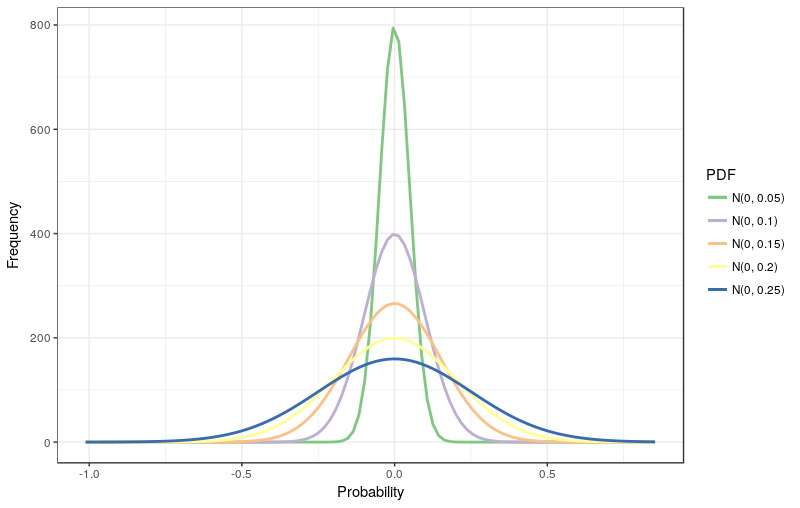
\includegraphics[width=0.8\textwidth]{img/gld_clustering/extra_images/5_gaussian.png}
    \caption{Gaussian (Normal) distributions used to generate the synthetic dataset.}
    \label{fig:5_gaussian}
\end{figure}

\begin{figure}[H]
    \centering
    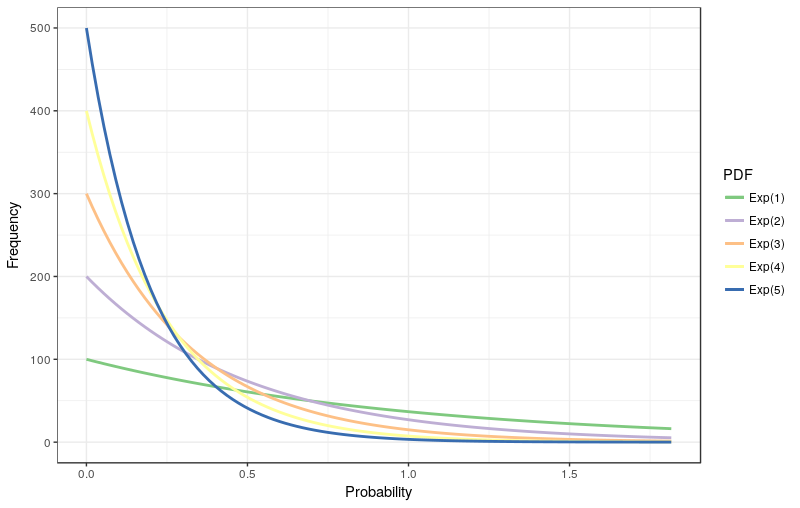
\includegraphics[width=0.8\textwidth]{img/gld_clustering/extra_images/5_exp.png}
    \caption{Exponential distributions used to generate the synthetic dataset.}
    \label{fig:5_exp}
\end{figure}

\begin{figure}[H]
    \centering
    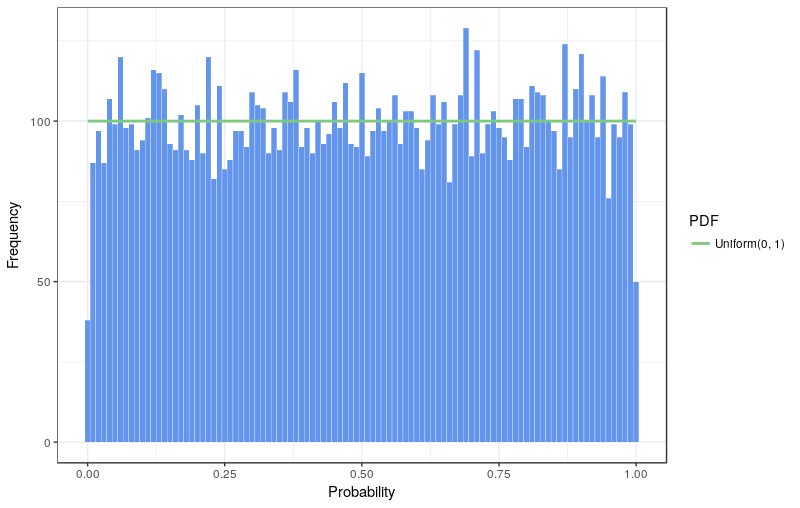
\includegraphics[width=0.8\textwidth]{img/gld_clustering/extra_images/uniform.png}
    \caption{Uniform distribution used to generate the synthetic dataset.}
    \label{fig:uniform}
\end{figure}

This dataset could be represented as a multidimensional array where for each position $x_{i}$, we have 1000 values $v_{j}$, equation \ref{eq:multi_array_datasetI}. In this case $i$ and $j$ vary from 1 to 1000 casually.

\begin{equation}\label{eq:multi_array_datasetI}
S(x_{i}, <v_{j}>) \quad i,j=1, 2.....1000
\end{equation}

The fitting algorithm proposed in subsection \ref{sub:fitting_gld} is applied over \ref{eq:multi_array_datasetI}. The good-of-fit test return that all the \textit{GLDs} are good fit for its corresponding distribution. As a result the dataset \ref{eq:multi_array3} is genarated. 

\begin{equation}\label{eq:multi_array3}
S(x_{i}, <\lambda_{1},\lambda_{2},\lambda_{3},\lambda_{4}>) \quad i=1.....1000
\end{equation}

\subsection{Clustering using $\lambda_{2}$, $\lambda_{3}$ and $\lambda_{4}$}\label{syntheticI_l234}

As we mention above, our idea is to test what happen if we use a simple k-means with euclidean distance over the $\lambda_{2}$, $\lambda_{3}$ and $\lambda_{4}$ values of the \textit{GLDs}. Similar to the paper \cite{Jiang2011}, as we use 11 \textit{PDFs} to generate the synthetic dataset I, we expect that the k-mean algorithm will return 11 clusters as well (one for each distribution). Then 11 is the number we use with the k-means algorithm.

In figure \ref{fig:dataset1_l2l3l4} and table \ref{tab:dataset1_l2l3l4} the distribution of the clusters returned by the k-means is shown.

\begin{figure}[H]
    \centering
    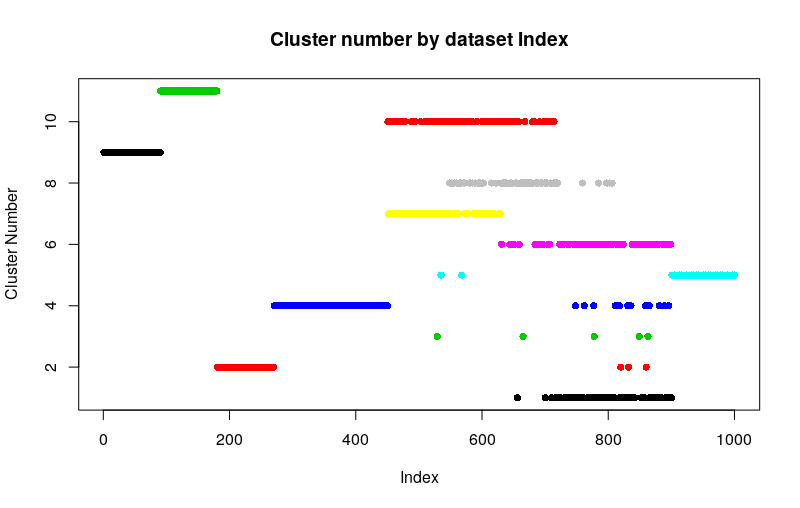
\includegraphics[width=0.8\textwidth]{img/gld_clustering/Dataset1/l2_l3_l4/intento_3/normal_exponential_uniform3.png}
    \caption{Distribution of the clusters using k-means over the $\lambda_{2}$, $\lambda_{3}$ and $\lambda_{4}$ values of the \textit{GLDs}.}
    \label{fig:dataset1_l2l3l4}
\end{figure}

\begin{table}[]
\centering
\caption{Distribution of the clusters using k-means over the $\lambda_{2}$, $\lambda_{3}$ and $\lambda_{4}$ values of the \textit{GLDs}.}
\label{tab:dataset1_l2l3l4}
\begin{tabular}{|c|c|c|}
\hline
Cluster & Type of Distribution & No. of Elements \\ \hline
1       & Exponential          & 82              \\ \hline
2       & Normal          & 93              \\ \hline
3       & Exponential          & 5             \\ \hline
4       & Normal               & 198              \\ \hline
5       & Uniform               & 102              \\ \hline
6       & Exponential               & 83             \\ \hline
7       & Exponential              & 91             \\ \hline
8       & Exponential          & 82              \\ \hline
9       & Normal          & 90               \\ \hline
10      & Exponential               & 84              \\ \hline
11      & Normal          & 90              \\ \hline
\end{tabular}
\end{table}

Remembered, the first 450 elements are normal distributions, the next 450 are exponential and the last 100 are uniform. Looking to those regions in general, the first observation is that we have 23 false positives, three in cluster 2, 18 in cluster 4 and two in cluster 5. The second observation is that, the normal distributions were grouped in 4 clusters (2, 4, 9 and 11), cluster 2 group perfectly it 90 elements with 2 false positives, clusters 9 and 11 group exactly its 90 elements each. The cluster 4 group the last 180 elements of the Normal distribution, with 18 false positives

The Uniform distribution was grouped totally in cluster 5, with two false positives as was mention above. The last observation is that the algorithm can't separate the 5 Exponential distributions, but this is not a bad result as we will show soon. 

In figures between \ref{fig:dataset1_l2l3l4_cl1} and \ref{fig:dataset1_l2l3l4_cl11} we show the \textit{PDFs} of all the distributions that belongs to the same cluster. If we take a look at figures \ref{fig:dataset1_l2l3l4_cl1}, \ref{fig:dataset1_l2l3l4_cl2}, \ref{fig:dataset1_l2l3l4_cl3}, \ref{fig:dataset1_l2l3l4_cl9}, \ref{fig:dataset1_l2l3l4_cl10} and \ref{fig:dataset1_l2l3l4_cl11} we see that the exponential distribution was well grouped. Really the problem is that the rate value of $0.05*i$ used to generate the exponential distribution does not have such a big difference between one and another.  

\begin{figure}[H]
    \centering
    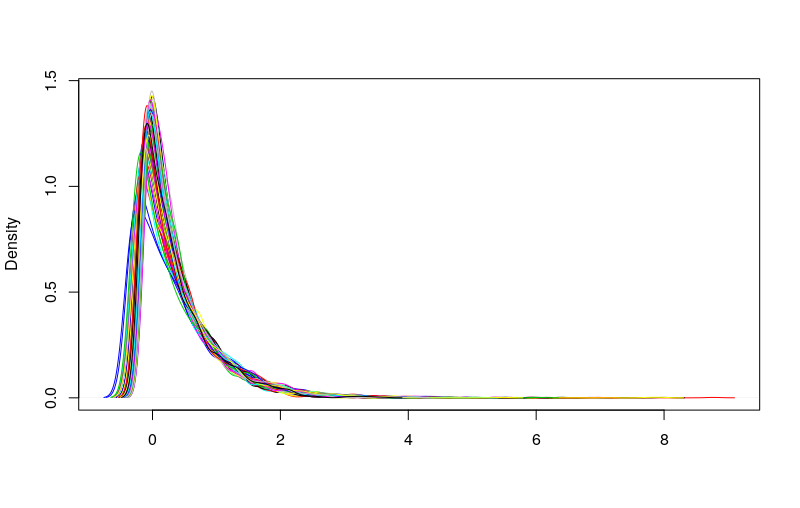
\includegraphics[width=0.8\textwidth]{img/gld_clustering/Dataset1/l2_l3_l4/intento_3/cluster1.png}
    \caption{Cluster 1 returned by the k-means over the $\lambda_{2}$, $\lambda_{3}$ and $\lambda_{4}$ values of the \textit{GLDs}, synthetic dataset I.}
    \label{fig:dataset1_l2l3l4_cl1}
\end{figure}

\begin{figure}[H]
    \centering
    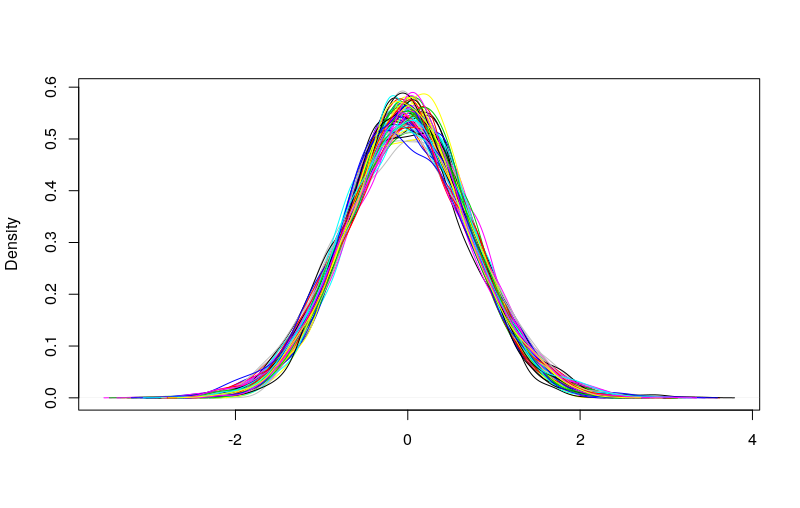
\includegraphics[width=0.8\textwidth]{img/gld_clustering/Dataset1/l2_l3_l4/cluster4.png}
    \caption{Cluster 2 returned by the k-means over the $\lambda_{2}$, $\lambda_{3}$ and $\lambda_{4}$ values of the \textit{GLDs}, synthetic dataset I.}
    \label{fig:dataset1_l2l3l4_cl2}
\end{figure}

\begin{figure}[H]
    \centering
    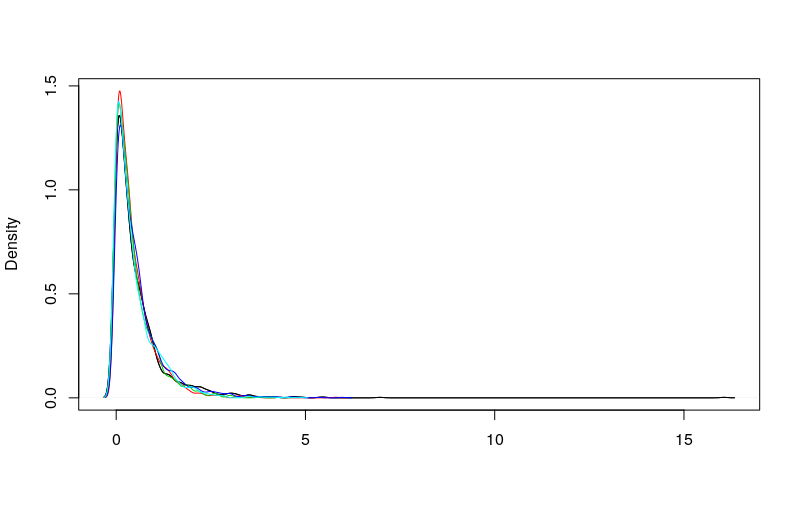
\includegraphics[width=0.8\textwidth]{img/gld_clustering/Dataset1/l2_l3_l4/intento_3/cluster3.png}
    \caption{Cluster 3 returned by the k-means over the $\lambda_{2}$, $\lambda_{3}$ and $\lambda_{4}$ values of the \textit{GLDs}, synthetic dataset I.}
    \label{fig:dataset1_l2l3l4_cl3}
\end{figure}

\begin{figure}[H]
    \centering
    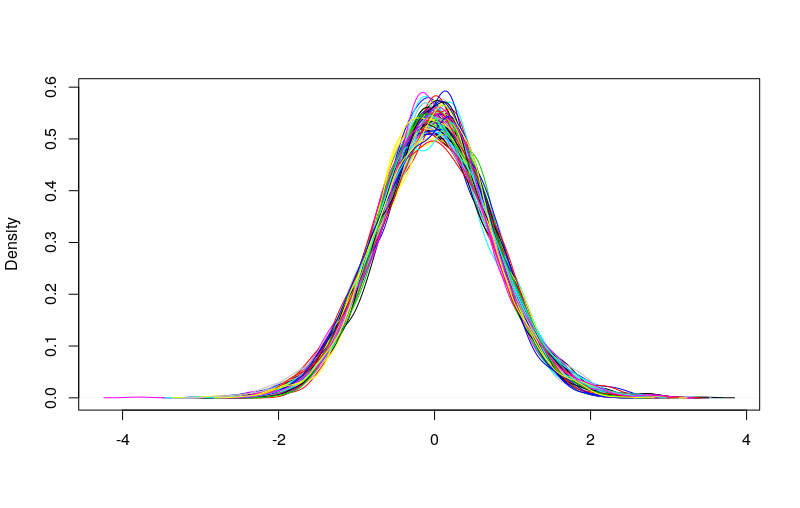
\includegraphics[width=0.8\textwidth]{img/gld_clustering/Dataset1/l2_l3_l4/cluster5.png}
    \caption{Cluster 4 returned by the k-means over the $\lambda_{2}$, $\lambda_{3}$ and $\lambda_{4}$ values of the \textit{GLDs}, synthetic dataset I.}
    \label{fig:dataset1_l2l3l4_cl4}
\end{figure}

\begin{figure}[H]
    \centering
    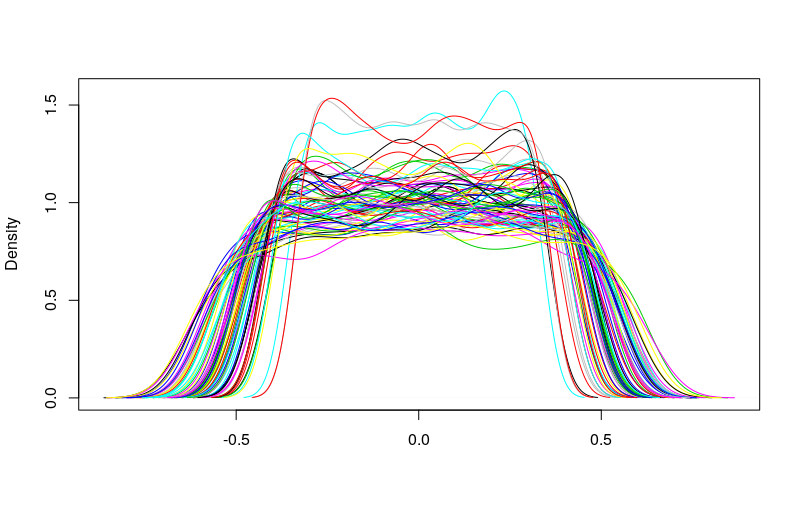
\includegraphics[width=0.8\textwidth]{img/gld_clustering/Dataset1/l2_l3_l4/cluster7.png}
    \caption{Cluster 5 returned by the k-means over the $\lambda_{2}$, $\lambda_{3}$ and $\lambda_{4}$ values of the \textit{GLDs}, synthetic dataset I.}
    \label{fig:dataset1_l2l3l4_cl5}
\end{figure}

\begin{figure}[H]
    \centering
    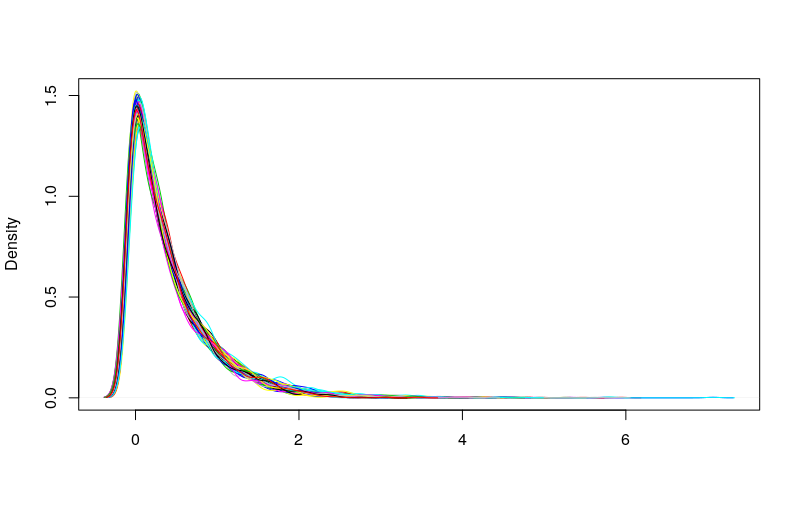
\includegraphics[width=0.8\textwidth]{img/gld_clustering/Dataset1/l2_l3_l4/intento_3/cluster6.png}
    \caption{Cluster 6 returned by the k-means over the $\lambda_{2}$, $\lambda_{3}$ and $\lambda_{4}$ values of the \textit{GLDs}, synthetic dataset I.}
    \label{fig:dataset1_l2l3l4_cl6}
\end{figure}

\begin{figure}[H]
    \centering
    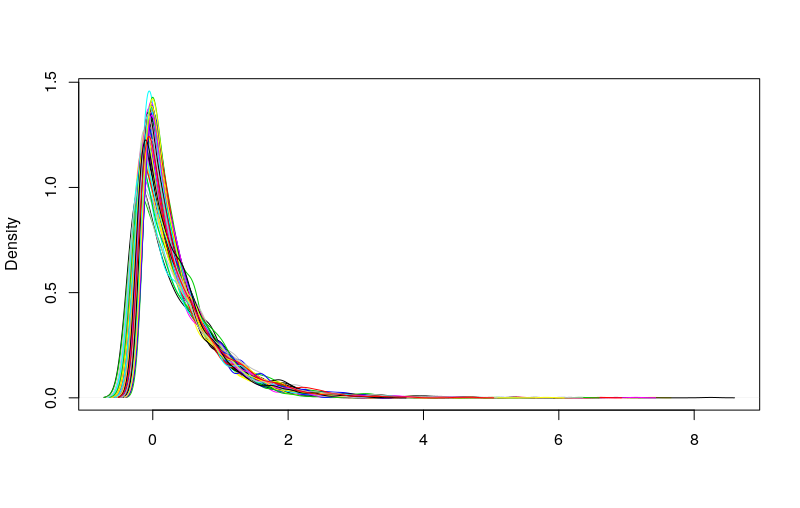
\includegraphics[width=0.8\textwidth]{img/gld_clustering/Dataset1/l2_l3_l4/intento_3/cluster7.png}
    \caption{Cluster 7 returned by the k-means over the $\lambda_{2}$, $\lambda_{3}$ and $\lambda_{4}$ values of the \textit{GLDs}, synthetic dataset I.}
    \label{fig:dataset1_l2l3l4_cl7}
\end{figure}

\begin{figure}[H]
    \centering
    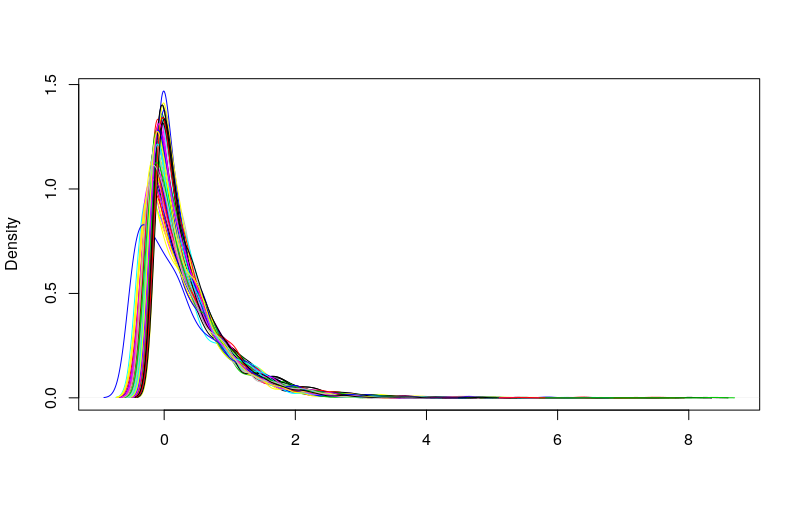
\includegraphics[width=0.8\textwidth]{img/gld_clustering/Dataset1/l2_l3_l4/intento_3/cluster8.png}
    \caption{Cluster 8 returned by the k-means over the $\lambda_{2}$, $\lambda_{3}$ and $\lambda_{4}$ values of the \textit{GLDs}, synthetic dataset I.}
    \label{fig:dataset1_l2l3l4_cl8}
\end{figure}

\begin{figure}[H]
    \centering
    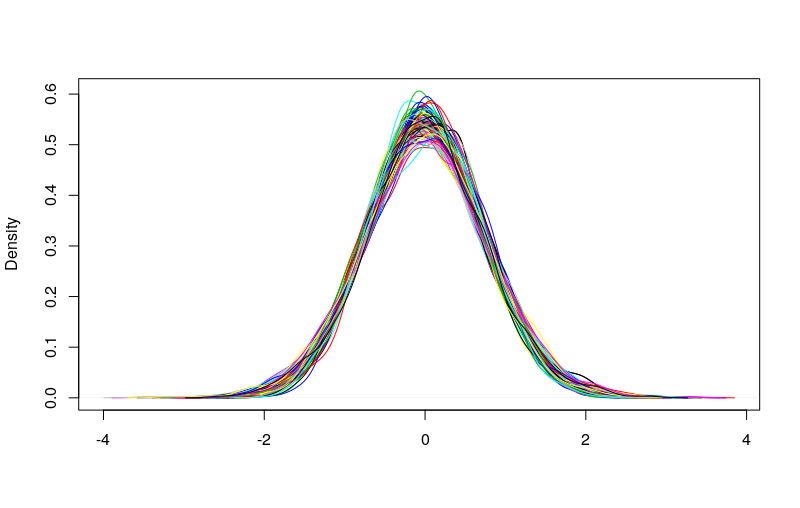
\includegraphics[width=0.8\textwidth]{img/gld_clustering/Dataset1/l2_l3_l4/intento_3/cluster9.png}
    \caption{Cluster 9 returned by the k-means over the $\lambda_{2}$, $\lambda_{3}$ and $\lambda_{4}$ values of the \textit{GLDs}, synthetic dataset I.}
    \label{fig:dataset1_l2l3l4_cl9}
\end{figure}

\begin{figure}[H]
    \centering
    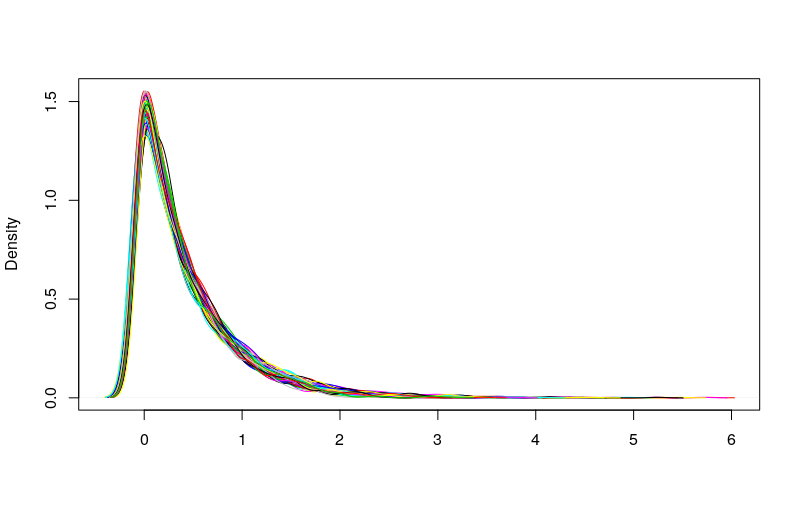
\includegraphics[width=0.8\textwidth]{img/gld_clustering/Dataset1/l2_l3_l4/intento_3/cluster10.png}
    \caption{Cluster 10 returned by the k-means over the $\lambda_{2}$, $\lambda_{3}$ and $\lambda_{4}$ values of the \textit{GLDs}, synthetic dataset I.}
    \label{fig:dataset1_l2l3l4_cl10}
\end{figure}

\begin{figure}[H]
    \centering
    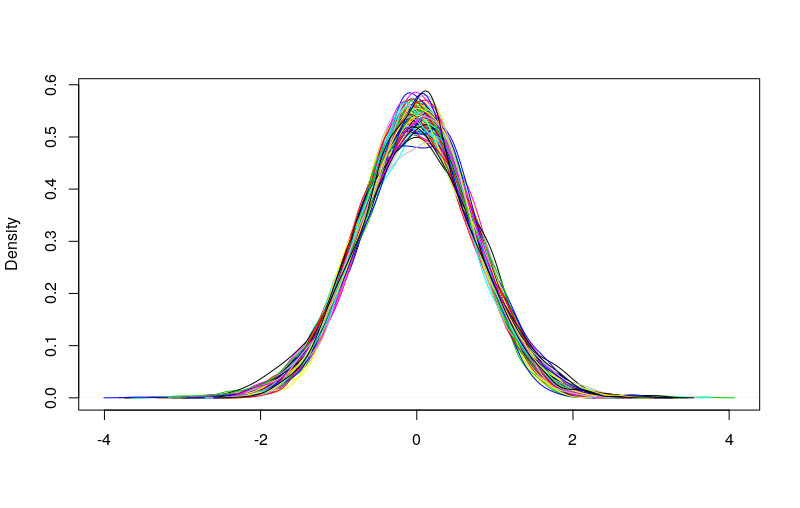
\includegraphics[width=0.8\textwidth]{img/gld_clustering/Dataset1/l2_l3_l4/intento_3/cluster11.png}
    \caption{Cluster 11 returned by the k-means over the $\lambda_{2}$, $\lambda_{3}$ and $\lambda_{4}$ values of the \textit{GLDs}, synthetic dataset I.}
    \label{fig:dataset1_l2l3l4_cl11}
\end{figure}

Another interesting result is show in figures \ref{fig:dataset1_l2l3l4_l3_l4} and \ref{fig:dataset1_l2l3l4_l3_l4_dividido}. As we can see, clusters 2, 4, 9 and 11 that represent the Normal distribution are all at the same region over the $\lambda_{3}$ and $\lambda_{4}$ space, near $\lambda_{3} = 0$ and $\lambda_{4} \in [0, 0.3]$. Similarly cluster 5, that represent the Uniform distribution is on the top left of the $\lambda_{3}$ and $\lambda_{4}$ space, $\lambda_{3} \in [0, 0.3]$ and $\lambda_{4} \in [0.7, 1.5]$. And finally the rest of the clusters that represent the Exponential distribution are distributed in the bottom of the $\lambda_{3}$ and $\lambda_{4}$ space, $\lambda_{3} \in [0.2, 7]$ and $\lambda_{4} \in [-0.1, 0.1]$. As we see in the rest of the thesis, this result is repeated in all the use cases.

\begin{figure}[H]
    \centering
    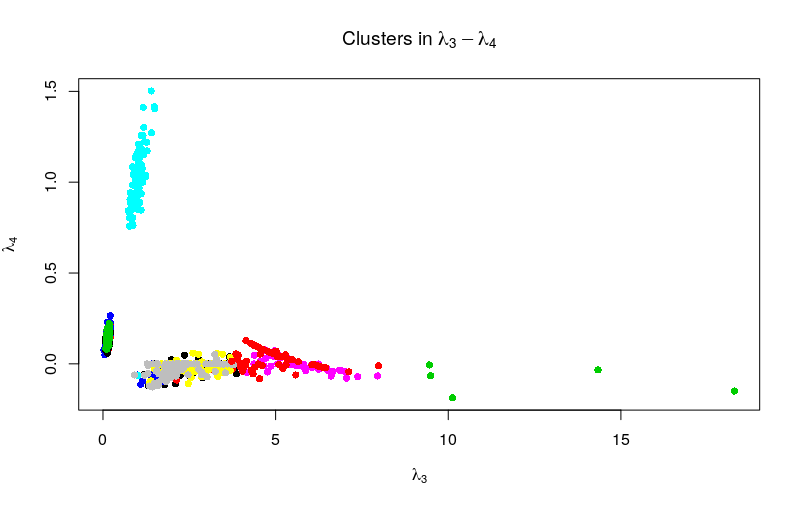
\includegraphics[width=0.8\textwidth]{img/gld_clustering/Dataset1/l2_l3_l4/intento_3/l3_l4.png}
    \caption{Distribution of the clusters over the $\lambda_{3}$ and $\lambda_{4}$ space.}
    \label{fig:dataset1_l2l3l4_l3_l4}
\end{figure}

\begin{figure}[H]
    \centering
    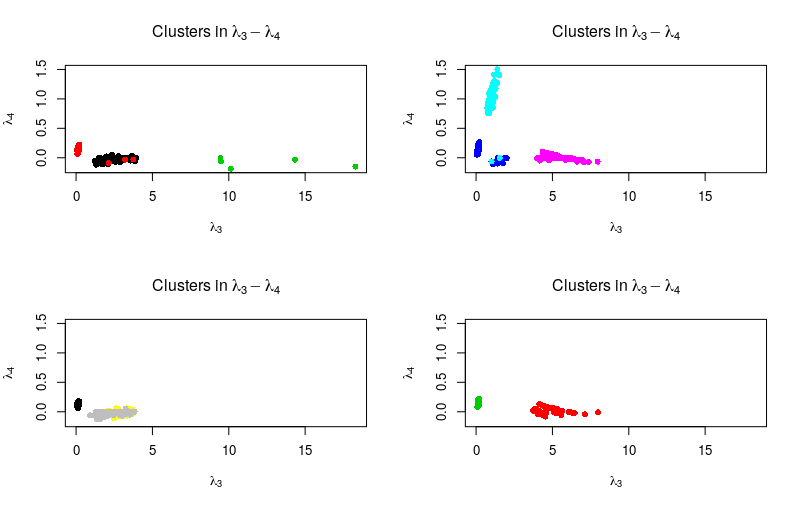
\includegraphics[width=0.8\textwidth]{img/gld_clustering/Dataset1/l2_l3_l4/intento_3/l3_l4_dividido.png}
    \caption{Distribution of the clusters over the $\lambda_{3}$ and $\lambda_{4}$ space. In the top left corner: clusters 1, 2 and 3. Top right corner: clusters 4, 5 and 6. Bottom left: clusters 7, 8 and 9. Bottom right: clusters 10 and 11.}
    \label{fig:dataset1_l2l3l4_l3_l4_dividido}
\end{figure}

\subsection{Clustering using $\lambda_{3}$ and $\lambda_{4}$}\label{syntheticI_l34}

In this section we proceed similar to section \ref{syntheticI_l234}, but the k-means algorithm run over $\lambda_{3}$ and $\lambda_{4}$. The distribution of the clusters is shown in figure \ref{fig:dataset1_l3l4} and table \ref{tab:dataset1_l3l4}.

\begin{figure}[H]
    \centering
    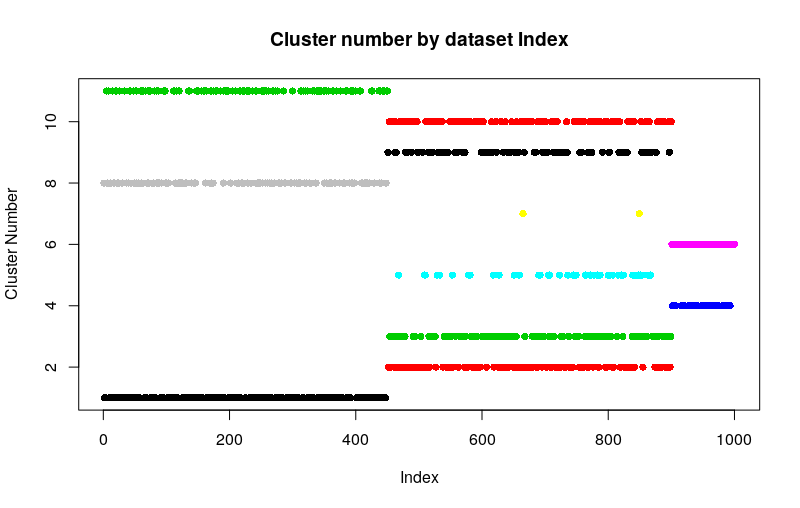
\includegraphics[width=0.8\textwidth]{img/gld_clustering/Dataset1/l3_l4/clusters_by_index.png}
    \caption{Distribution of the clusters using k-means over the $\lambda_{3}$ and $\lambda_{4}$ values of the \textit{GLDs}.}
    \label{fig:dataset1_l3l4}
\end{figure}

\begin{table}[]
\centering
\caption{Distribution of the clusters using k-means over the $\lambda_{3}$ and $\lambda_{4}$ values of the \textit{GLDs}.}
\label{tab:dataset1_l3l4}
\begin{tabular}{|c|c|c|}
\hline
Cluster & Type of Distribution & No. of Elements \\ \hline
1       & Normal          & 197              \\ \hline
2       & Exponential          & 118              \\ \hline
3       & Exponential          & 110             \\ \hline
4       & Uniform               & 35              \\ \hline
5       & Exponential               & 41              \\ \hline
6       & Uniform               & 65             \\ \hline
7       & Exponential              & 2             \\ \hline
8       & Normal          & 131              \\ \hline
9       & Exponential          & 74               \\ \hline
10      & Exponential               & 105              \\ \hline
11      & Normal          & 122              \\ \hline
\end{tabular}
\end{table}
 
 
As we don't use $\lambda_{2}$ here, is clear that the algorithm can't distinguish the distributions by its standard deviation. But, as the shape of the \textit{GLD} is defined by $\lambda_{3}$ and $\lambda_{4}$, what we expect is that the algorithm can separate the objects by type of distribution. As we see in figure \ref{fig:dataset1_l3l4} this is exactly what we get, there is no any false positive in this case, the three regions (Normal, Exponential and Uniform) are identified by the k-means.

Clusters 1, 8 and 11 group all the Normal distributions, clusters 4 and 6 group the Uniform and the rest group the Exponential.

In the $\lambda_{3}$ and $\lambda_{4}$ space the behavior is very similar at the one we get in subsection \ref{syntheticI_l234}, figures \ref{fig:dataset1_l3l4_l3_l4} and \ref{fig:dataset1_l3l4_l3_l4_dividido}. Again the distributions are concentrated near the same $(\lambda_{3}, \lambda_{4})$ values.

\begin{figure}[H]
    \centering
    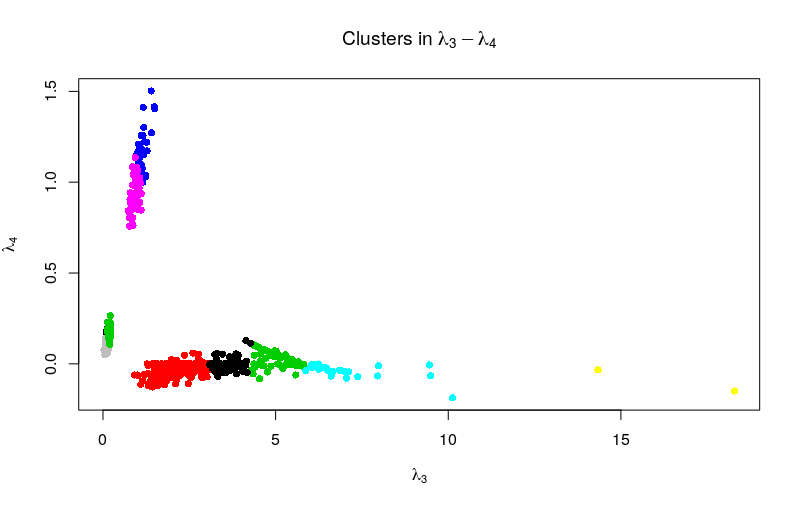
\includegraphics[width=0.8\textwidth]{img/gld_clustering/Dataset1/l3_l4/l3_l4.png}
    \caption{Distribution of the clusters over the $\lambda_{3}$ and $\lambda_{4}$ space.}
    \label{fig:dataset1_l3l4_l3_l4}
\end{figure}

\begin{figure}[H]
    \centering
    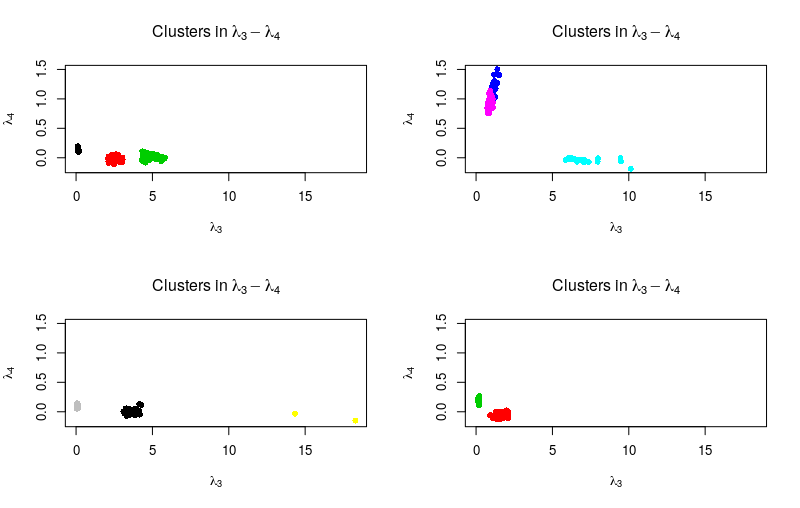
\includegraphics[width=0.8\textwidth]{img/gld_clustering/Dataset1/l3_l4/l3_l4_dividido.png}
    \caption{Distribution of the clusters over the $\lambda_{3}$ and $\lambda_{4}$ space. In the top left corner: clusters 1, 2 and 3. Top right corner: clusters 4, 5 and 6. Bottom left: clusters 7, 8 and 9. Bottom right: clusters 10 and 11.}
    \label{fig:dataset1_l3l4_l3_l4_dividido}
\end{figure}

%\subsection{Effectiveness of the Clustering}

\section{Synthetic Data II}\label{sec:synthetic_II}
The second synthetic dataset is similar to the first one, here we include 5 Gamma distributions, between the Exponential and the Uniform, figure \ref{fig:5_gamma}. The shape of the Gamma distribution is $i$, with $i=1, 2, 3, 4, 5$. This dataset have 1450 objects, where the first 450 were sampled from a Gaussian distributions, the next 450 from an Exponential, the next 450 are Gamma, and the last 100 from a Uniform distribution. As we use 16 different distributions, this is the number of clusters to be used with the k-means algorithm. 

\begin{figure}[H]
    \centering
    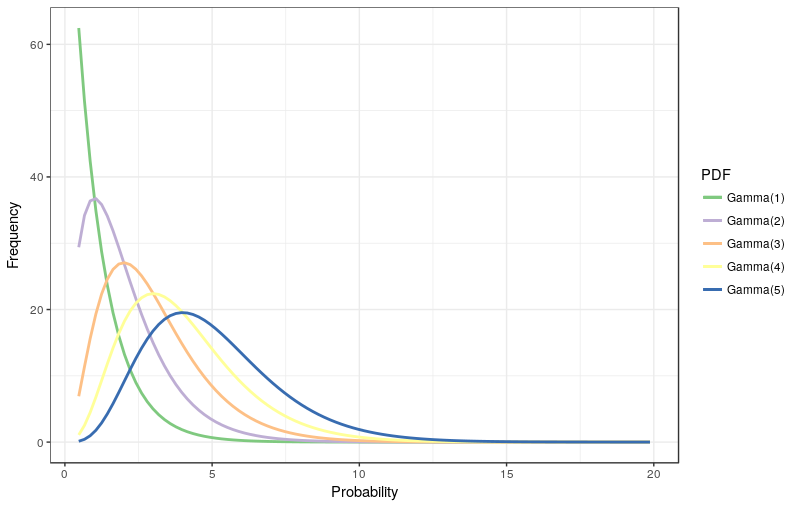
\includegraphics[width=0.8\textwidth]{img/gld_clustering/extra_images/5_gamma.png}
    \caption{Gamma distributions used to generate the synthetic dataset.}
    \label{fig:5_gamma}
\end{figure}

Similar to the dataset I, the fitting algorithm proposed in subsection \ref{sub:fitting_gld} is applied over dataset II. The good-of-fit test return that all the \textit{GLDs} are good fit for its corresponding distribution.

\subsection{Clustering using $\lambda_{2}$, $\lambda_{3}$ and $\lambda_{4}$}\label{syntheticII_l234}

The distribution of the clusters returned by the k-means algorithm is shown in figure \ref{fig:dataset2_l2l3l4} and table \ref{tab:dataset2_l2l3l4}.

\begin{figure}[H]
    \centering
    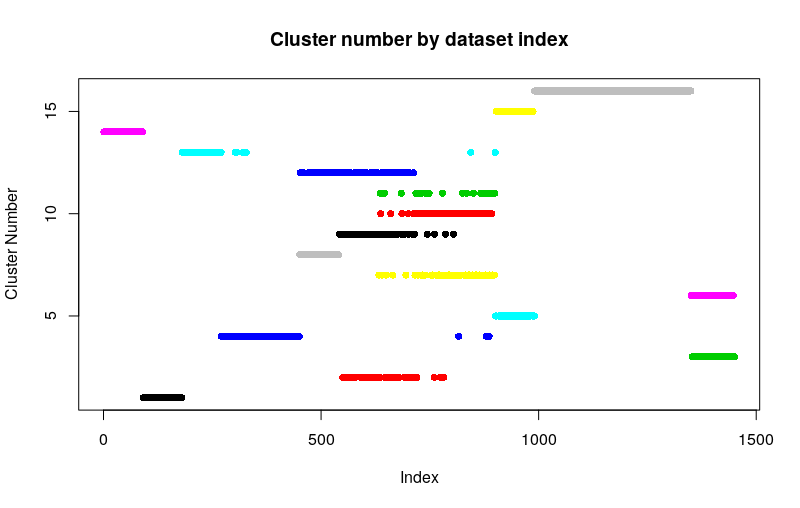
\includegraphics[width=0.8\textwidth]{img/gld_clustering/Dataset2/nuevo/clusters_by_index.png}
    \caption{Distribution of the clusters using k-means over the $\lambda_{2}$, $\lambda_{3}$ and $\lambda_{4}$ values of the \textit{GLDs}.}
    \label{fig:dataset2_l2l3l4}
\end{figure}

\begin{table}[]
\centering
\caption{Distribution of the clusters using k-means over the $\lambda_{2}$, $\lambda_{3}$ and $\lambda_{4}$ values of the \textit{GLDs}.}
\label{tab:dataset2_l2l3l4}
\begin{tabular}{|c|c|c|}
\hline
Cluster & Type of Distribution & No. of Elements \\ \hline
1       & Normal          & 90              \\ \hline
2       & Exponential          & 44              \\ \hline
3       & Uniform          & 45             \\ \hline
4       & Normal               & 179              \\ \hline
5       & Gamma               & 60             \\ \hline
6       & Uniform               & 55            \\ \hline
7       & Exponential              & 87            \\ \hline
8       & Exponential          & 58              \\ \hline
9       & Exponential          & 67               \\ \hline
10      & Exponential               & 74              \\ \hline
11      & Exponential          & 25              \\ \hline
12       & Exponential              & 90             \\ \hline
13       & Normal          & 96              \\ \hline
14       & Normal          & 90              \\ \hline
15      & Gamma               & 30              \\ \hline
16      & Gamma          & 360              \\ \hline
\end{tabular}
\end{table}

In general the results are very similar to the results of the section \ref{sec:synthetic_I}, but we get less false positives, 5 in total. 3 false positives in cluster 4 and 2 false positves in cluster 13. The normal distribution was groping again in for clusters: 1, 4, 13 and 14. The uniform distribution was grouping in clusters 3 and 6 without false positives. The gamma distribution introduced here was grouped in clusters 5, 15 and 16, without false positives. And finally the rest of the clusters are for the exponential distribution.

The projection of the clusters over the $\lambda_{3}$ and $\lambda_{4}$ space is show in figure \ref{fig:dataset2_l2l3l4_l3_l4}. The two clusters of the uniform distribution are located again in the top-left region of the figure. The normal distribution is located in the same place, near $\lambda_{3} = 0$ and $\lambda_{4} \in [0, 0.3]$. The exponential distribution is distributed in the bottom of the $\lambda_{3}$ and $\lambda_{4}$ space. The gamma distribution is overlapped together with the normal distribution.

\begin{figure}[H]
    \centering
    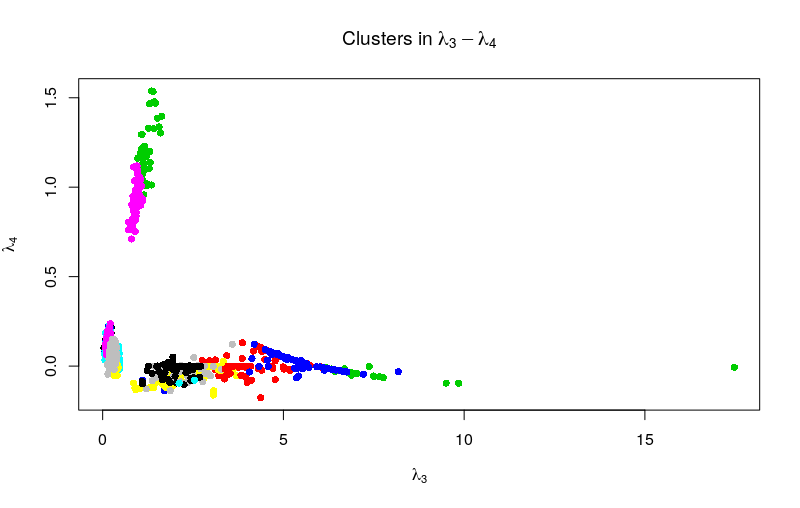
\includegraphics[width=0.8\textwidth]{img/gld_clustering/Dataset2/nuevo/l3_l4.png}
    \caption{Distribution of the clusters over the $\lambda_{3}$ and $\lambda_{4}$ space.}
    \label{fig:dataset2_l2l3l4_l3_l4}
\end{figure}

%\begin{figure}[H]
%    \centering
%    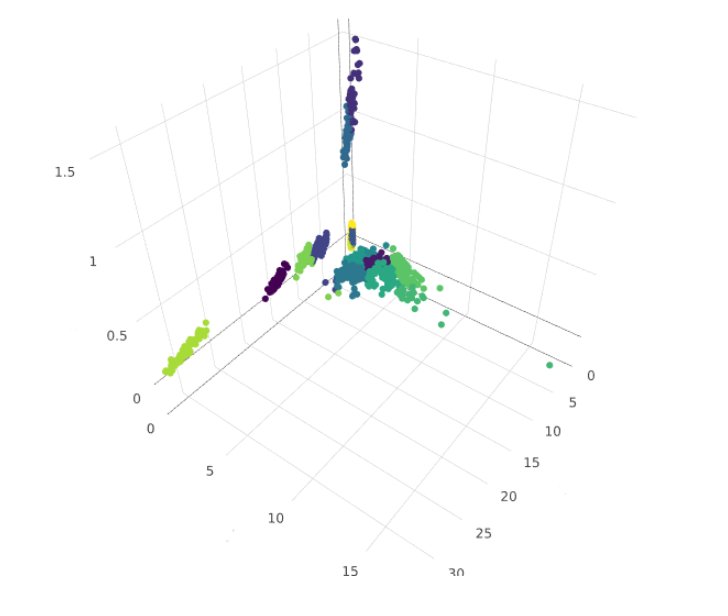
\includegraphics[width=0.8\textwidth]{img/gld_clustering/Dataset2/nuevo/l2_l3_l4_cortado.png}
%    \caption{Distribution of the clusters over the $\lambda_{2}$,  $\lambda_{3}$ and $\lambda_{4}$ space.}
%    \label{fig:dataset2_l2l3l4_l2_l3_l4}
%\end{figure}

\subsection{Clustering using $\lambda_{3}$ and $\lambda_{4}$}\label{syntheticI_l34}

The distribution of the clusters returned by the k-means when using the values of $\lambda_{3}$ and $\lambda_{4}$ to group the second synthetic dataset are shown in figure \ref{fig:dataset2_l3l4} and table \ref{tab:dataset2_l3l4}.
 
A few false positives are observed in clusters 5, 6 and 12, but nothing to worry about. Again the regions of the four distribution families are perfectly separated by the algorithm. 
 
\begin{table}[]
\centering
\caption{Distribution of the clusters using k-means over the $\lambda_{3}$ and $\lambda_{4}$ values of the \textit{GLDs}.}
\label{tab:dataset2_l3l4}
\begin{tabular}{|c|c|c|}
\hline
Cluster & Type of Distribution & No. of Elements \\ \hline
1       & Exponential          & 64              \\ \hline
2       & Exponential          & 126              \\ \hline
3       & Exponential          & 1             \\ \hline
4       & Exponential               & 57              \\ \hline
5       & Gamma               & 83             \\ \hline
6       & Normal               & 139            \\ \hline
7       & Uniform              & 67            \\ \hline
8       & Gamma          & 148              \\ \hline
9       & Gamma          & 108               \\ \hline
10      & Exponential               & 75              \\ \hline
11      & Exponential          & 80              \\ \hline
12       & Normal              & 112             \\ \hline
13       & Exponential          & 44              \\ \hline
14       & Normal          & 201              \\ \hline
15      & Gamma               & 112              \\ \hline
16      & Uniform          & 33              \\ \hline
\end{tabular}
\end{table}
 
 \begin{figure}[H]
    \centering
    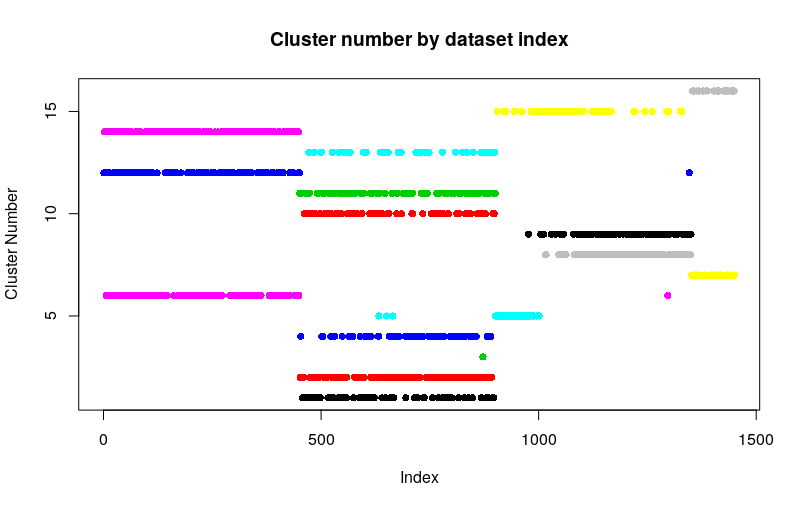
\includegraphics[width=0.8\textwidth]{img/gld_clustering/Dataset2/nuevo/l3_l4/clusters_by_index.png}
    \caption{Distribution of the clusters using k-means over the $\lambda_{2}$, $\lambda_{3}$ and $\lambda_{4}$ values of the \textit{GLDs}.}
    \label{fig:dataset2_l3l4}
\end{figure}

The projection of the clusters over the $\lambda_{3}$ and $\lambda_{4}$ space is show in figure \ref{fig:dataset2_l3l4_l3_l4}.

\begin{figure}[H]
    \centering
    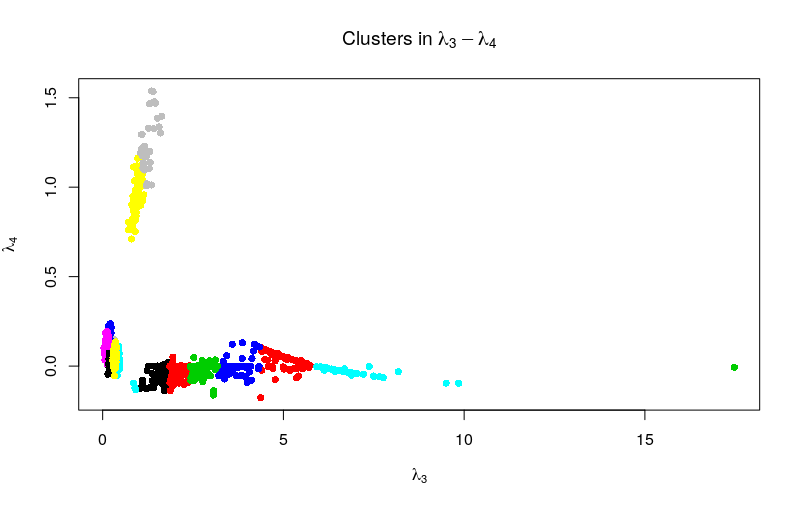
\includegraphics[width=0.8\textwidth]{img/gld_clustering/Dataset2/nuevo/l3_l4/l3_l4.png}
    \caption{Distribution of the clusters over the $\lambda_{3}$ and $\lambda_{4}$ space.}
    \label{fig:dataset2_l3l4_l3_l4}
\end{figure}

%\subsection{Effectiveness of the Clustering}

\section{Summary}\label{sec:clustering_summary}

In this Chapter, we explore clustering uncertain data based on the similarity between their distributions. The idea is to answer the \textbf{RQ.1} \textit{"how to group the output of the UQ process based on the similarity of the uncertainty?"}. The hypothesis enunciated at the beginning of the Chapter was tested against two synthetic datasets, and the results corroborate that we can group uncertain data based in the $\lambda_{i}$ values of the \textit{GLDs} that describe the data.

As a second result we test that, when using $\lambda_{2}$, $\lambda_{3}$ and $\lambda_{4}$ the separations of the different distributions of the dataset was almost perfect with a few false positives; and when using $\lambda_{3}$ and $\lambda_{4}$ all the elements of the same family are grouping together without consider the difference in the standard deviation. Both results are exactly what we expect.

Another important result of this Chapter, is that if we look at the clustering technique proposed here and compare it with the state-of-the-art, our approach is a competitive one. For example, in the approach proposed by \cite{Jiang} the computational cost of its algorithm depend of two factors, the fit of the distributions using Kernel Density Estimation (KDE) and the computation of the KL-divergence (the distance measure used in its approach). Both factors are computationally intensive. In our approach we substitute KDE by \textit{GLD} fit, that is most costly form the computational point of view; but at the same time we substitute the KL-divergence by simple distance comparisons in $\mathbf{R}$ and $\mathbf{R^2}$. On the other hand, some limitations of the KL-divergence approach as: (i) the \textit{PDF} of every uncertain object to be clustered need to be defined in the same domain and (ii) the needs to select an appropriate kernel to fit the data using KDE, are solved with the use of the \textit{GLD}.

All of this observation join with the rest of the advantage of the use of the \textit{GLD} to quantify the uncertainty, make our approach far superior to those reported in the literature.    


%\section{Ideas por si son necesarias}
%
%\subsection{The Gaussian (Normal) Distribution}
%The Gaussian (Normal) distribution is probably the most used and also the most well-known distribution. Many groups follow this type of pattern. That's why it's widely used in business, statistics and in government bodies like the FDA:
%\begin{itemize}
%\item Heights of people.
%\item Measurement errors.
%\item Blood pressure.
%\item Points on a test.
%\item IQ scores.
%\item Salaries.
%\end{itemize}
%
%The PDF of the Normal Distribution is represented in equation \ref{eq:gaussian_distribution}
%
%\begin{equation}\label{eq:gaussian_distribution}
%f(x) = \frac{1}{{ \sqrt {2\pi \sigma} }}e^{{{ - \left( {x - \mu } \right)^2 } \mathord{\left/ {\vphantom {{ - \left( {x - \mu } \right)^2 } {2\sigma ^2 }}} \right. \kern-\nulldelimiterspace} {2\sigma ^2 }}}
%\end{equation}
%
%where:
%\begin{itemize}
%\item $\mu$ is the mean or expectation of the distribution (and also its median and mode),
%\item $\sigma$ is the standard deviation, and
%\item $\sigma^2$ is the variance.
%\end{itemize}
%
%To generate a synthetic normal distribution we need to specify the number of elements we want (e.g. 1000) and the mean and standard deviation. In \textit{R} for example we can use a function \textbf{\textit{rnorm(1000, 0, 2)}} to generate 1000 elements of a normal distribution with mean $\mu = 0$ and standard deviation $\sigma = 2$, figure \ref{fig:normal_sample}.
%
%\begin{figure}[H]
%    \centering
%    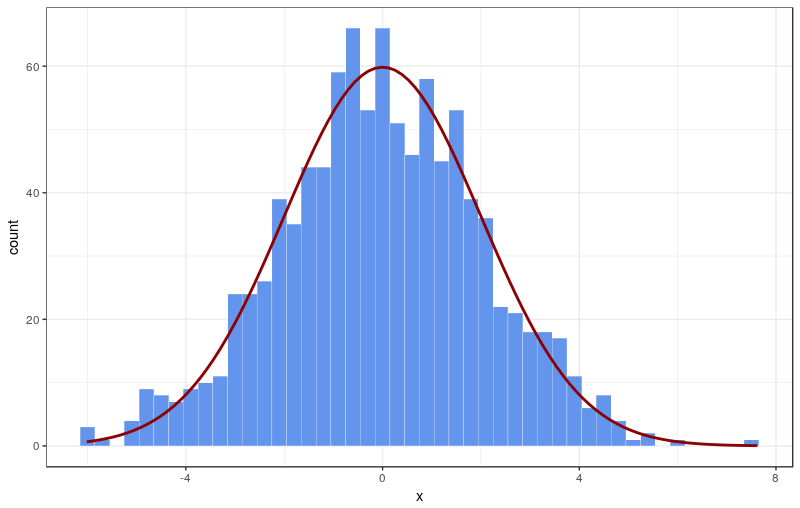
\includegraphics[width=0.8\textwidth]{img/gld_clustering/extra_images/normal_0_2.png}
%    \caption{Normal distribution generated using the \textit{R} function \textbf{\textit{rnorm(1000, 0, 2)}} with mean $\mu = 0$ and standard deviation $\sigma = 2$.}
%    \label{fig:normal_sample}
%\end{figure}
%
%\subsection{The Exponential Distribution}
%\begin{equation}\label{eq:exponential_distribution}
%  f(x) =
%  \begin{cases}
%    \lambda e^{-\lambda x} & \text{$x >= 0 $} \\
%    0 & \text{$x < 0$}
%  \end{cases}
%\end{equation}
%
%\begin{figure}[H]
%    \centering
%    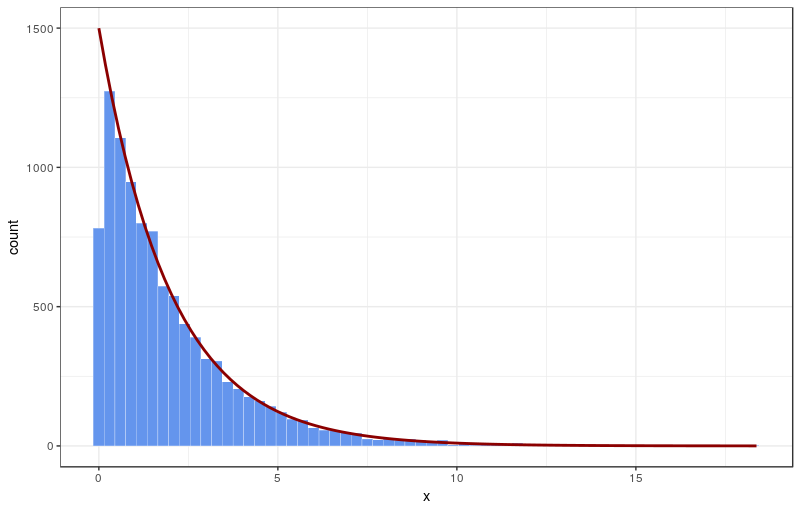
\includegraphics[width=0.8\textwidth]{img/gld_clustering/extra_images/exp_05.png}
%    \caption{Exponential distribution generated using the \textit{R} function \textbf{\textit{rexp(1000, 0.5)}} with rate $\lambda = 0.5$.}
%    \label{fig:normal_sample}
%\end{figure}
%
%\subsection{The Uniform Distribution}
%\begin{equation}\label{eq:uniform_distribution}
%  f(x) =
%  \begin{cases}
%    \frac{1}{b-a} & \text{$a < x < b$} \\
%    0 & \text{$x < a$ or $x > b$}
%  \end{cases}
%\end{equation}
%
%\begin{figure}[H]
%    \centering
%    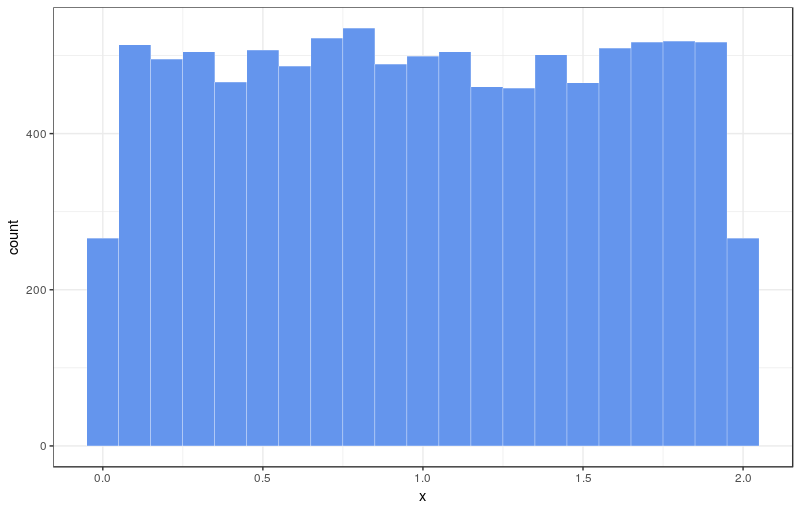
\includegraphics[width=0.8\textwidth]{img/gld_clustering/extra_images/unif_0_2.png}
%    \caption{Uniform distribution generated using the \textit{R} function \textbf{\textit{runif(1000, 0, 2)}} in the interval $[0, 2]$.}
%    \label{fig:normal_sample}
%\end{figure}
%
%\subsection{The Gamma Distribution}
%\begin{equation}\label{eq:gamma_distribution}
%  f(x) =
%  \begin{cases}
%    \frac{x^{\alpha-1}e^{\frac{-x}{\theta}}}{\Gamma(\alpha)\theta^{\alpha}} & \text{$x >= 0 $} \\
%    0 & \text{$x < 0$}
%  \end{cases}
%\end{equation}
%
%\begin{figure}[H]
%    \centering
%    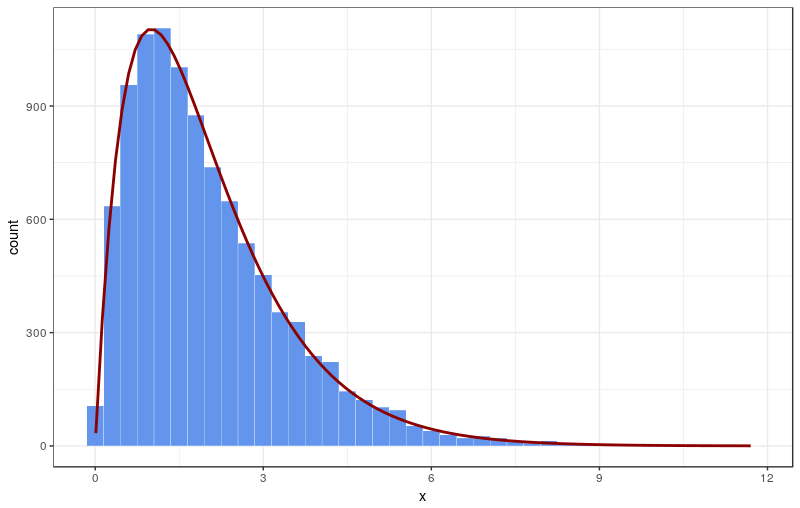
\includegraphics[width=0.8\textwidth]{img/gld_clustering/extra_images/gamma_2.png}
%    \caption{Gamma distribution generated using the \textit{R} function \textbf{\textit{rgamma(1000, 2)}} with shape $\alpha = 2$.}
%    \label{fig:normal_sample}
%\end{figure}

\chapter{Kriging of the GLD parameters}\label{cap:kriging}

\begin{tcolorbox}
\textbf{RQ2.} what is the uncertainty in some spatio-temporal locations not previously analyzed?
\end{tcolorbox}


\section{Spatio-temporal Interpolation}
However, adding the temporal domain implies that variability in space and time must be modelled, which is more complicated than modelling purely spatial or purely temporal variability \cite{Graler2016}.

\section{Kriging over GLD}

\section{Use Case}

\section{Conclusions}

%\chapter{UQMS Data Model}\label{cap_data_model}

\section{Introduction}

\section{SaViMe}

\section{UQMS Data Model}

\section{UQMS Operations}

%\chapter{Implementation of the UQMS in Tensorflow}\label{cap_tensorflow}

\section{Why Tensorflow}

\subsection{Variables in Tensorflow}

\subsection{Operations in Tensorflow}

%\chapter{Case Study: Seismic Example}\label{cap_seismic}

\chapter[Use Cases]{Use Cases}\label{cap:use_cases}

In the present chapter we are going to test the UQMS in three different scenarios, spatial only domain, section \ref{Wave Propagation} , spatio-temporal domain, section \ref{spatio_temporal}, and finally a multidisciplinary system, section \ref{NASA}. 

\section{Case Study:  Wave Propagation Problem}\label{Wave Propagation}

The first one is a geophysical tests for wave propagation problems

As a first case study we use the “HPC4E Seismic Test Suite”, a collection of four 3D models and sixteen associated tests that can be downloaded freely at the project's website (https://hpc4e.eu/downloads/datasets-and-software ). The models include simple cases that can be used in the development stage of any geophysical imaging practitioner (developer, tester ...) as well as extremely large cases that can only be solved in a reasonable time using ExaFLOPS supercomputers. The models are generated to the required size by means of a Matlab/Octave script and hence can be used by users of any OS or computing platform. The tests can be used to benchmark and compare the capabilities of different and innovative seismic modelling approaches, hence simplifying the task of assessing the algorithmic and computational advantages that they pose. %\cite{deLaPuente2015}

In our case, we are going to use the “HPC4E Seismic Test Suite” as a case study of the porposed UQMS. As we mention in the introduction of this chapter this model is a spatial only domain problem, because we are going to consider a multidimentional array as an Input and a multidimentional array as an output, but of them time independet.

\subsection{Mathematical Formulation}

\subsection{Model and Dataset Description}
The models have been designed as a set of 16 layers with constant physical properties. The top layer delineates the topography and the other 15 different layer interface surfaces or horizons. In the following, an interface horizon is associated with properties that apply to the layer that exists between itself and the immediately next layer horizon. The model covers an area of 10 x 10 x 5 km, with maximum topography at about 500 m and maximum depth at about 4500 m. The layer horizons have been sampled very finely with 1.6667 m spacing so that a highly accurate representation can be honored at high frequencies. For simulation schemes based on unstructured grids, the layer horizons can be used easily to constrain model blocks. For simulation schemes based upon Cartesian grids, a simple script is provided that can generate 3D grids for any desired spatial sampling. Table \ref{layers_constants} shows the properties of each of the layers included in the models. %\cite{deLaPuente2015}

\begin{table}[]
\centering
\caption{Layer constant properties and their depth range. “Star” layers are only used in the flat case, in substitution of their non-star equivalents}
\label{layers_constants}
\begin{tabular}{|l|l|l|l|l|l|}
\hline
\multicolumn{1}{|c|}{\textbf{\begin{tabular}[c]{@{}c@{}}Layer\\ Id\end{tabular}}} & \multicolumn{1}{c|}{\textbf{\begin{tabular}[c]{@{}c@{}}Vp\\ (m/s)\end{tabular}}} & \multicolumn{1}{c|}{\textbf{\begin{tabular}[c]{@{}c@{}}Vs\\ (m/s)\end{tabular}}} & \multicolumn{1}{c|}{\textbf{\begin{tabular}[c]{@{}c@{}}Density\\ (Kg/m3)\end{tabular}}} & \multicolumn{1}{c|}{\textbf{\begin{tabular}[c]{@{}c@{}}Max. depth\\ (m)\end{tabular}}} & \multicolumn{1}{c|}{\textbf{\begin{tabular}[c]{@{}c@{}}Min. depth\\ (m)\end{tabular}}} \\ \hline
1 & 1618.92 & 500.00 & 1966.38 & -135.55 & -476.35 \\ \hline
2 & 1684.08 & 765.49 & 1985.88 & 41.50 &  -394.90 \\ \hline
3 &  &  &  &  &  \\ \hline
4 &  &  &  &  &  \\ \hline
5 &  &  &  &  &  \\ \hline
6 &  &  &  &  &  \\ \hline
7 &  &  &  &  &  \\ \hline
8 &  &  &  &  &  \\ \hline
9 &  &  &  &  &  \\ \hline
10 &  &  &  &  &  \\ \hline
11 &  &  &  &  &  \\ \hline
12 &  &  &  &  &  \\ \hline
13 &  &  &  &  &  \\ \hline
14 &  &  &  &  &  \\ \hline
15 &  &  &  &  &  \\ \hline
16 &  &  &  &  &  \\ \hline
2* &  &  &  &  &  \\ \hline
3* &  &  &  &  &  \\ \hline
\end{tabular}
\end{table}

\subsection{Adding uncertainty into the model}

The “HPC4E Seismic Test Suite” does not provide uncertainty sources, because all the input parameters of the model have fixed values. Then, to the purpose of our work we need to add some uncertainties into the inputs. Let's suppose the variable ${V_{p}}$ is uncertain. As this variable have 16 different values, one for each layer, we can consider it as a random vector, equation \ref{random_vector_vp}. We associate to each of the $V_{{p}_{i}}$ a Normal distribution with ${\mu}_{i}$ equal to the value reported in Table \ref{layers_constants} and $\sigma=2$.
\begin{equation}\label{random_vector_vp}
V_{p}=<V_{{p}_{i}},\mathcal{N}({\mu}_{i},{\sigma}_{i})>
\end{equation}

\section{Case Study: Austin, queso library}\label{spatio_temporal}

\section{Case Study: Multidisciplinary System (NASA)}\label{NASA}

\section{Case Study: Spatio-temporal Nicholson-Bailey model}
Este esta en el software uqlab, en la carpeta Doc Manuals

%\chapter[Validation]{Validation}\label{Validation}


% ---

% ----------------------------------------------------------
% Finaliza a parte no bookmark do PDF
% para que se inicie o bookmark na raiz
% e adiciona espaço de parte no Sumário
% ----------------------------------------------------------
\phantompart

% ---
% Conclusão
% ---
\chapter[Conclusions and Future Works]{Conclusions and Future Works}\label{cap:conclusions}
Large-scale spatio-temporal simulations produce a huge amount of data that need to be interpreted in order to assess the simulation quality in different regions of space-time. Querying these data poses a great challenge due to their volume and different data distributions. In order to solve this problem, 
in this paper we propose SUQ$^2$, a general approach to answer uncertainty quantification queries. 

The approach uses \textit{GLD} that enables the representation of a spatio-temporal simulation output using a single functional formalism. By modeling each spatio-temporal point by a GLD instance, we can synthesize the region in a number of clusters, represented by their centroid GLD function. From this basis, queries can be answered by combining the centroids in a spatio-time region into GLD-mixture functions. Moreover, by using information entropy techniques, a value can be assigned that represents the uncertainty in a region. The proposed approach is implemented in a workflow that can be extended to solve new UQ queries.

We ran extensive experiments using a seismic use case. The results showed that GLD representation of the data is valid on $85 \%$ of the dataset. Other extensions of the GLD formalism, such as EGLD \cite{Karian2011}, can be evaluated to improve the GLD dataset coverage. Moreover, we showed that the computed centroid function is a good representation of the function instances in its cluster. Additionally, we use the Kolmogorov-Smirnov test to evaluate the quality of the GLD mixture. The p-value, larger than 0.05, assures that the results of the mixture is a good representation of the raw data in the region. Finally, the adoption of the Information Entropy technique was validated by showing the correspondence of the computed values with the uncertainty in the spatio-temporal regions. 

To the best of our knowledge, this is the first work to use GLD as the basis for answering UQ queries in spatio-temporal regions and to compile a series of techniques to produce a query answering workflow.

\section{Revisiting the Research Questions}

\section{Significance and Limitations}

\section{Open Problems and Future Work}
Some of the future directions we are interested in pursuing were mentioned above. For example, in Section \ref{useCaseClustering} we mention that for the purpose of this paper we select \textit{k-means} as the clustering algorithm to be used. This arbitrary selection needs to be studied, and some algorithms implemented to provide an automatic way to cluster the \textit{GLDs}, based on the shapes described in Section \ref{gldShape}.

In Section \ref{useCaseQualityofFit}, there is a region where the \textit{GLD} does not fit well the dataset. If we want to provide a general purpose computational approach for \textit{forward propagation} we need to further investigate this issue.

The use of Information Entropy to quantify the uncertainty is very powerful. However, when applied on clusters of PDFs, such as the GLD, it observes the information variation as a function of the PDF definition, in the case of GLD this is given by its for $\lambda$ parameters. In this context, a complete region modeled by a single GLD function would have a very low information entropy value. This, however would not express the uncertainty modeled by the GLD function, which could be very high. The outcome of the information entropy evaluation must be interpreted by the user. 

\section{Final Considerations}

\subsection*{Acknowledgments}
This work has been funded by CNPq, CAPES, FAPERJ, Inria (SciDISC project) and the European Commission (HPC4E H2020 project) and performed (for E. Pacitti and P. Valduriez) in the context of the Computational Biology Institute (www.ibc-montpellier.fr) and for (F. Porto, H. Lustosa and N. Lemus) in the context of the DEXL Laboratory (dexl.lncc.br)  at LNCC.

%\chapter[Future Works]{Future Works}\label{FutureWorks}

\begin{itemize}
\item Use of other distribution families in the regions where the GLD is not valide.
\item Implement the same flow using other distribution families.
\item Optimize all the process using Spark or other Big data System.
\item Implement all the algorithms as operators inside SAVIME.
\end{itemize}
% ---

% ----------------------------------------------------------
% ELEMENTOS PÓS-TEXTUAIS
% ----------------------------------------------------------
\postextual
% ----------------------------------------------------------

% ----------------------------------------------------------
% Referências bibliográficas
% ----------------------------------------------------------
\bibliography{MyCollection}

% ----------------------------------------------------------
% Glossário
% ----------------------------------------------------------
%
% Consulte o manual da classe abntex2 para orientações sobre o glossário.
%
%\glossary

% ----------------------------------------------------------
% Apêndices
% ----------------------------------------------------------

% ---
% Inicia os apêndices
% ---
\begin{apendicesenv}

% Imprime uma página indicando o início dos apêndices
\partapendices

% Inclusão dos arquivos referentes aos apêndices
% ----------------------------------------------------------
\chapter{Título do apêndice A}\label{apendiceA}

\lipsum[50]

\section{Título da seção}

Aqui temos uma seção dentro do Apêndice.

\begin{figure}
    \begin{center}
        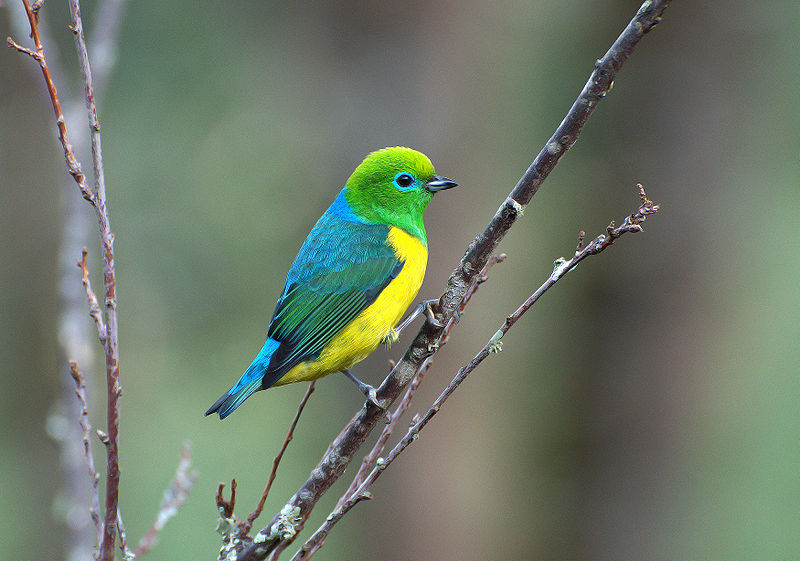
\includegraphics[width=12cm]{img/abntex2-modelo-livro-bandeirinha}
        \caption{Legenda para a figura.}
        \label{rotulo1}
    \end{center}
\end{figure}
\chapter{Título do apêndice B}\label{apendiceB}

\lipsum[55-57]

\chapter{Título do apêndice C}\label{apendiceC}

%\lipsum[9] 

% ----------------------------------------------------------

\end{apendicesenv}
% ---

% ----------------------------------------------------------
% Anexos
% ----------------------------------------------------------

% ---
% Inicia os anexos
% ---
\begin{anexosenv}

% Imprime uma página indicando o início dos anexos
\partanexos

% Inclusão dos arquivos referentes aos anexos
% ----------------------------------------------------------
\chapter{Título do anexo A}\label{anexoA}

\lipsum[23-24]

\section{Título da seção}

Aqui temos uma seção dentro do Anexo.

\lipsum[25]

\chapter{Título do anexo B}\label{anexoB}

%\lipsum[76-77]
\chapter{Título do anexo C}\label{anexoC}

\lipsum[55-57]
% ----------------------------------------------------------

\end{anexosenv}

%---------------------------------------------------------------------
% INDICE REMISSIVO
%---------------------------------------------------------------------
\phantompart
\printindex
%---------------------------------------------------------------------

\end{document}
